\documentclass[a4paper,oneside,parskip=half,numbers=noenddot]{scrbook}
\textwidth=14.7cm
\textheight=22.1cm
%\hoffset=5.8754pt % enable if using letterpaper

\pdfminorversion=7 %use a more current pdf version to support better graphics inclusions

\usepackage{comment}
\excludecomment{comment-2016}
\usepackage{framed}
\usepackage{verbatim}
\usepackage[utf8]{inputenc}
\usepackage[T1]{fontenc}
\usepackage{lmodern}
\usepackage{longtable}
\usepackage{multicol}
\usepackage{multirow}
\usepackage{array}
\usepackage{color} % for latexdiff
\usepackage[normalem]{ulem} % for latexdiff
\newcolumntype{P}[1]{>{\raggedright\arraybackslash}p{#1}} % use column type 'P' instead of 'p' for non-justified text
\usepackage[shortlabels]{enumitem}
\setlist{itemsep=-1mm, topsep=-1pt, partopsep=0pt}

\newlist{judging_items}{itemize}{1} %redefine itemize for the freestyle judging grid to fit
\setlist[judging_items]{label=\textbullet,leftmargin=*, labelsep=0.7mm,itemsep=-1mm, topsep=-6pt, partopsep=-5pt}
% \usepackage[nenglish]{babel}


% turning off part numbering in the backmatter
% parts will still go to the TOC
\makeatletter
\g@addto@macro\backmatter{\setcounter{secnumdepth}{-2}}
\makeatother



% Numberings, table of Contents, bookmarks
\usepackage{hyperref} % clickable table of contents, index in pdf files (must be loaded before minitoc)
\usepackage{minitoc} % for table of contents per part
\usepackage{remreset} % for removal of counter resets
\usepackage[numbered]{bookmark} % customize PDF bookmarks
\renewcommand{\mtcgapbeforeheads}{0pt}
\renewcommand{\mtcgapafterheads}{0pt}


%TOC customization
\usepackage[tocindentauto]{tocstyle} % prettier TOC
\usetocstyle{allwithdot} %use 'KOMAlike" if you don't want dots
\settocstylefeature [-1] {entryvskip} {15pt}
\settocstylefeature [0] {entryvskip} {10pt}
\settocstylefeature [0] {entryhook} {\hspace{18pt} }
\mtcsettitle{parttoc}{Contents} %renames the part TOC to match main TOC
\usepackage[titles]{tocloft}
\renewcommand*\cftsecnumwidth{3em}

% %don't reset page numbers ever
\makeatletter
\def\pagenumbering#1{%
  \gdef\thepage{\csname @#1\endcsname \c@page}}
\makeatother


%%%headings
\usepackage[markcase=ignoreuppercase,autooneside]{scrlayer-scrpage} %better headings without uppercase TOC heading
\usepackage{titlesec}
%\usepackage[nouppercase]{scrpage2} %better headings without uppercase TOC heading

\titlespacing\section{0pt}{12pt plus 4pt minus 2pt}{0pt plus 2pt minus 2pt}
\titlespacing\subsection{0pt}{12pt plus 4pt minus 2pt}{0pt plus 2pt minus 2pt}
\titlespacing\subsubsection{0pt}{12pt plus 4pt minus 2pt}{0pt plus 2pt minus 2pt} %save space after (sub)section headers


\pagestyle{scrheadings}
\clearscrheadfoot %clear all header and footer styles to allow custimization
\cfoot[\pagemark]{\pagemark} %pagenumbers in footer
\makeatletter
\let\Oldpart\part
\newcommand{\parttitle}{}
\renewcommand{\part}[1]{\Oldpart{#1}\renewcommand{\parttitle}{#1}}
\renewcommand{\chaptermark}[1]{\markboth{#1}{}}

\renewcommand*{\chapterpagestyle}{headings} %display headers on first page of chapters

\chead[]{
  \ifnum\value{chapter}>0
    \thepart \ \parttitle -- \leftmark
  \else
    \thepart \ \parttitle 
  \fi
  }
\makeatother

\newcommand\singlechapter[1]{%if a part only has a single chapter in it use \singlechapter{} otherwise use the normal \chapter{}
    \begin{mtchideinmaintoc}
        \addstarredchapter{#1}
        \chapter*{#1}
        \markright{\thepart\ #1}
    \end{mtchideinmaintoc}}


\setcounter{tocdepth}{-1} % only includes parts and chapters (not sections) in main TOC
\mtcsetdepth{parttoc}{1} % only includes chapters and sections (not sub or subsubsections) in part TOCs
\setcounter{secnumdepth}{3} % makes subsubsections numbered
\renewcommand{\thepart}{\arabic{part}} % arabic part numbering
\renewcommand{\thechapter}{\arabic{part}\Alph{chapter}} % make chapters numbered with part and then letter
%\renewcommand{\thesection}{\arabic{part}.\arabic{section}} % replace chapter number with part number in sections 
\makeatletter
\@addtoreset{chapter}{part} % reset chapter numbering for each part
\@addtoreset{section}{part} % reset section numbering for each part
%\@removefromreset{section}{chapter} % don't reset section numbering in new chapters
\makeatother
\hypersetup{
    colorlinks,
    citecolor=black,
    filecolor=black,
    linkcolor=black,
    urlcolor=black
}
% If you get the error: "Argument of \contentsline has an extra }"
% This is because hyperref and minitoc don't work perfectly together.
% Just continue to typeset ignoring all errors.
% Un-commenting the following line should supress errors.
% \batchmode
% Make sure to re-comment this line after typeseting to see future errors.
% Then typeset again and the error should be gone.
% This has to be done for each tex file (chapter) that contains a TOC.



\newcommand{\unit}[1]{\ensuremath{\, \mathrm{#1}}} % use \unit{km} in math mode for better units

\newcommand{\oldrule}[1]{}
%\newcommand{\oldrule}[1]{\framebox{#1}} % defines the \oldrule command to allow for nice styling

\usepackage{graphicx}
\graphicspath{{img/}}
\usepackage{wrapfig}
\usepackage{pict2e}

% Documentation of gitinfo:
% http://ftp.fernuni-hagen.de/ftp-dir/pub/mirrors/www.ctan.org/macros/latex/contrib/gitinfo/gitinfo.pdf
%Simple instructions: copy "hooks" directory into ".git" directory
\usepackage{gitinfo2}
\renewcommand{\thesection}{\arabic{part}\alph{chapter}.\arabic{section}} % replace chapter number with part number in sections

\begin{document}

\begin{titlepage}
\centering
\ \\
\vspace{5cm}
{\Huge IUF Standard Skills List}
\vspace{5mm}

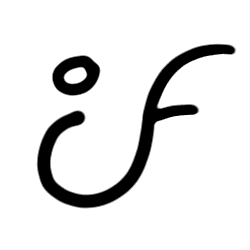
\includegraphics{../img/iuf-logo}

\vspace{5mm}
{\huge International Unicycling Federation}

\vspace{70mm}
Prepared by the IUF Rulebook Committee.

\vspace{5mm}
{\small Copyright \copyright\ 2015 by the International Unicycling Federation, Inc. All rights reserved.} \\
\small{Last Revision 2012.}

\end{titlepage}

\setcounter{chapter}{5}\setcounter{part}{6}
\chapter{List of Standard Skills \label{chap:freestyle_std-skills-list}}

\section{General Remarks About Standard Skill Riding  }
Only figures listed in the following skills list can be used for the assembly of Standard Skill routines.

\subsection{Riding Position}
Unless stated differently in a figure description, it is to be executed with the rider seated and with both feet on the pedals.

\subsection{Body Form}
The rider must show proper body form and shall not change this form during the execution of the entire figure.
Proper body form must also be shown for the figure before and after transitions, even if not listed on the judging sheet.
The body form may be relaxed when not performing figures, except for figures before and after transitions.

\subsection{Riding Direction}
Unless stated differently, all riding figures are to be performed riding forward, this being the direction in which the rider faces.

\subsection{Pattern}
Unless stated differently in a figure description, it is to be executed in a line.
Exceptions are mounts, stationary skills and transitions, axis skills, single and counted short skills, which can be executed at any spot in the riding area.

\subsection{Transitions, And Single Short Skills}
Unless stated differently in the description of a transition, it starts and ends with the rider seated with both feet on the pedals.
Before and after transitions, and single short skills entered on the score sheet as figures, at least one revolution of the wheel must be ridden in the start and end positions.
If the start or end position of a transition or single short skill is a counted short skill, that skill must be executed at least 50\% as described, whether or not it is listed on the judging sheet.

\textbf{Example 1:} For the transition ``Riding to Seat in Front'', the rider must ride at least one full revolution of the wheel with the seat in front.

\textbf{Example 2:} For the single short skill, 180$^\circ$ uni spin to idling 1ft, the rider must idle one foot $2 \frac{1}{2}$ cycles.

\subsection{Axis Skills}
Unless stated differently in the description, it starts and ends with the rider seated with both feet on the pedals.
Before axis skills entered on the score sheet as figures, at least one revolution of the wheel must be ridden in the start position.
After axis skills, at least one revolution of the wheel must be ridden.
The ending position is not required to be the same as the starting position.

\subsection{Mounts}
Unless stated differently in the description of a mount, it is to end with the rider seated with both feet on the pedals.
After all mounts listed on the judging sheet as figures, at least one full revolution of the wheel must be ridden in the end position.
For mounts ending in counted short skills, the skill must be executed at least 50\% as described, whether or not it is listed on the judging sheet.

\textbf{Example:} For the Side Mount, the rider must ride at least one full revolution of the wheel in the riding position after mounting.

\subsection{Seat Out Figures}
Unless stated differently in seat out figures, the rider shall have no contact with the seat other than one hand holding the seat.
The hand holding the seat as well as the corresponding arm shall be extended away from the rider's body and shall not touch any part of the rider's body.

\subsection{One Foot Figures}
Unless stated differently in one foot figures, the free foot is to be placed on the frame so that there is no contact between the free foot and any rotating part of the unicycle.

\subsection{Wheel Walk Figures}
Unless stated differently in wheel walk figures, the feet are to push only the tire, and shall have no contact with the pedals or crank arms.

\subsection{Coasting}
Unless stated differently in coasting figures, the feet are to have no contact with any rotating part of the unicycle (pedals, crank arms, or tire).

\subsection{Transitions, Single Short Skills, Mounts Involving Seat Out Skills}
Unless stated differently in the description of the figure, those beginning or ending in seat out skills are allowed to have one or both hands touching the seat, and the seat touching the body for the final or first hop, idle, or revolution.
This includes, but is not limited to: unispins to seat out skills, transitions into and out of seat in front or back, leg around skills, side ride to seat in front, transitions out of seat drag in front or back, hopping wheel to pedals.

\subsection{Transitions To/From Stand Up Wheel Walk}
In all transition skills from/to stand up wheel walk position, a second foot may briefly touch the wheel during the transition, but only one foot pushes the wheel forward.
Unless clearly stated in the description, the rider must perform stand up wheel walk forward.

\subsection{Spins And Pirouettes}
The rider must make a minimum of three full rotations for spins and pirouettes.
Spins must be ridden around a fixed point and must not exceed a 1 meter diameter.
If rider rotates more than required minimum number, the last required rotations are judged for spins.
Pirouettes must be executed on 1 spot and the pedals may not move backward or forward during the pirouette.
If rider rotates more than required minimum number, the first required rotations are judged for pirouettes.

\subsection{Leg Around Skills}
All variations may begin or end with feet on the cranks or pedals and begin or end either riding, idling, or hopping unless otherwise specified.

\subsection{Idling Figures}
In idling figures, a minimum of 5 consecutive cycles (back and forth motions) must be executed.

\subsection{Twisting Figures}
In twisting figures, a minimum of 5 consecutive cycles (side to side motions) must be executed.

\subsection{Stillstands}
The minimum time for stillstands is 3 seconds.

\subsection{Hopping Figures}
In hopping figures, a minimum of 5 consecutive hops must be executed.

\section{Standard Skill Scores and Descriptions}
The following descriptions are meant to explain the correct way to execute the skills.
Any illustrations are intended to clarify the descriptions.
If illustrations and descriptions disagree, the descriptions always apply.

\textbf{Abbreviations Used In This List:}
\begin{center}
\begin{tabular}{l l l p{2cm} l l l}
fwd & = & forward & & c & = & circle \\
ext & = & extended & & 1ft & = & one foot \\
bwd & = & backward & & 8 & = & figure eight \\
frh & = & freehand & & ww & = & wheel walk \\
\end{tabular}
\end{center}
\newpage

\subsection{Riding Skills}
\renewcommand{\arraystretch}{1.5}
\begin{longtable}{|r|c|p{4cm}|p{8cm}|c|}
\hline
1 & a & riding  & Riding (sitting on seat, facing forward). & 1.0 \\ 
\hline
  & b & riding - c  & Riding in a circle (sitting on seat, facing forward). & 1.3 \\ 
\hline
  & c & riding - 8  & Riding in a figure eight sitting on seat, facing forward).  & 1.5 \\ 
\hline
2 & a & riding holding seatpost, 1 hand & Riding while leaning forward and with one hand holding the seatpost under the seat. & 1.3 \\ 
\hline
  & b & riding holding seatpost, 1 hand - c & Riding in a circle while leaning forward and with one hand holding the seatpost under the seat. & 1.6 \\ 
\hline
  & c & riding holding seatpost, 1 hand - 8 & Riding in a figure 8 while leaning forward and with one hand holding the seatpost under the seat. & 1.9 \\ 
\hline
  & d & riding holding seatpost, 2 hands  & Riding while leaning forward and with both hands holding the seatpost under the seat. & 1.4 \\ 
\hline
  & e & riding holding seatpost, 2 hands - c  & Riding in a circle while leaning forward and with both hands holding the seatpost under the seat. & 1.8 \\ 
\hline
  & f & riding holding seatpost, 2 hands - 8  & Riding in a figure 8 while leaning forward and with both hands holding the seatpost under the seat. & 2.0 \\ 
\hline
3 & a & riding bwd  & Riding backward.  & 2.5 \\ 
\hline
  & b & riding bwd - c  & Riding in a circle backward.  & 3.1 \\ 
\hline
  & c & riding bwd - 8  & Riding backward in a figure eight.  & 3.6 \\ 
\hline
4 & a & seat in front, seat against body  & Riding with seat held in front of the rider. The seat or hand holding the seat may rest against the rider.  & 2.0 \\ 
\hline
  & b & seat in front & Riding with seat held in front of the rider.  & 2.3 \\ 
\hline
  & c & seat in front - c & Riding in a circle with seat held in front of the rider.  & 2.9 \\ 
\hline
  & d & seat in front - 8 & Riding in a figure eight with seat held in front of the rider.  & 3.3 \\ 
\hline
  & e & seat in front frh, seat against body  & Riding with seat held out in front of the rider. Neither hand touches the seat and the seat post is held between the rider's legs. The seat may rest against the rider. & 3.3 \\ 
\hline
  & f & seat in front frh & Riding with seat held in front of the rider. Neither hand touches the seat and the seat post is held between the rider's legs.  & 3.7 \\ 
\hline
  & g & seat in front frh - c & Riding in a circle with seat held in front of the rider. Neither hand touches the seat and the seat post is held between the rider's legs.  & 4.3 \\ 
\hline
  & h & seat in front frh - 8 & Riding in a figure eight with seat held in front of the rider. Neither hand touches the seat and the seat post is held between the rider's legs.  & 4.8 \\ 
\hline
5 & a & seat in front bwd, seat against body  & Riding backward with seat held out in front of the rider. The seat or hand holding the seat may rest against the rider. & 3.4 \\ 
\hline
  & b & seat in front bwd & Riding backward with seat held out in front of the rider. & 3.6 \\ 
\hline
  & c & seat in front bwd - c & Riding backward in a circle with seat held out in front of the rider. & 4.1 \\ 
\hline
  & d & seat in front bwd - 8 & Riding backward in a figure eight with seat held out in front of the rider. & 4.7 \\ 
\hline
  & e & seat in front bwd frh, seat against body  & Riding backward with seat held out in front of the rider. Neither hand touches the seat and the seat post is held between the rider's legs. The seat may rest against the rider.  & 4.0 \\ 
\hline
  & f & seat in front bwd frh & Riding backward with seat held out in front of the rider. Neither hand touches the seat and the seat post is held between the rider's legs. & 4.5 \\ 
\hline
  & g & seat in front bwd frh - c & Riding backward in a circle with seat held out in front of the rider. Neither hand touches the seat and the seat post is held between the rider's legs. & 5.2 \\ 
\hline
6 & a & seat in back, seat against body & Riding with the seat held out behind the rider. The seat or the hand holding the seat may rest against the rider. & 2.2 \\ 
\hline
  & b & seat in back  & Riding with the seat held out behind the rider. & 2.5 \\ 
\hline
  & c & seat in back - c  & Riding in a circle with the seat held out behind the rider. & 3.1 \\ 
\hline
  & d & seat in back - 8  & Riding in a figure eight with the seat held out behind the rider. & 3.6 \\ 
\hline
7 & a & seat in back bwd, seat against body & Riding backward with the seat held out behind the rider. The seat or the hand holding the seat may rest against the rider.  & 3.5 \\ 
\hline
  & b & seat in back bwd  & Riding backward with the seat held out behind the rider.  & 3.9 \\ 
\hline
  & c & seat in back bwd - c  & Riding backward in a circle with the seat held out behind the rider.  & 4.5 \\ 
\hline
  & d & seat in back bwd - 8  & Riding backward in a figure eight with the seat held out behind the rider.  & 5.1 \\ 
\hline
8 & a & seat on side, seat against body & Riding with the seat held out to the side of the rider. The seat or the hand holding the seat may rest against the rider. & 3.4 \\ 
\hline
  & b & seat on side, seat against body - c & Riding in a circle with the seat held out to the side of the rider. The seat or the hand holding the seat may rest against the rider. & 3.2 \\ 
\hline
  & c & seat on side  & Riding with the seat held out to the side of the rider. & 4.1 \\ 
\hline
  & d & seat on side - c  & Riding in a circle with the seat held out to the side of the rider. & 3.9 \\ 
\hline
9 & a & seat on side bwd, seat against body & Riding backward with the seat held out to the side of the rider. The seat or the hand holding the seat may rest against the rider.  & 4.3 \\ 
\hline
  & b & seat on side bwd  & Riding backward with the seat held out to the side of the rider.  & 4.6 \\ 
\hline
  & c & seat on side bwd - c  & Riding backward in a circle with the seat held out to the side of the rider.  & 4.4 \\ 
\hline
10  & a & stomach on seat, 1 hand on seat & Riding with the abdomen on the seat. One hand holds onto the seat.  & 2.1 \\ 
\hline
  & b & stomach on seat & Riding with the abdomen on the seat, frh. & 2.3 \\ 
\hline
  & c & stomach on seat - c & Riding in a circle with the abdomen on the seat, frh. & 2.9 \\ 
\hline
  & d & stomach on seat - 8 & Riding in a figure eight with the abdomen on the seat, frh. & 3.3 \\ 
\hline
11  & a & stomach on seat bwd & Riding backward with the abdomen on the seat, hands free. & 3.8 \\ 
\hline
  & b & stomach on seat bwd - c & Riding backward in a circle with the abdomen on the seat, hands free. & 4.4 \\ 
\hline
  & c & stomach on seat bwd - 8 & Riding backward in a figure eight with the abdomen on the seat, hands free. & 4.9 \\ 
\hline
12  & a & chin on seat, 1 hand on seat  & Riding with no part of the body other than the chin touching the back of the seat. One hand may touch the seat. & 3.5 \\ 
\hline
  & b & chin on seat  & Riding with no part of the body other than the chin touching the back of the seat, freehanded.  & 4.0 \\ 
\hline
  & c & chin on seat - c  & Riding in a circle with no part of the body other than the chin touching the back of the seat, freehanded.  & 4.6 \\ 
\hline
  & d & chin on seat - 8  & Riding in a figure eight with no part of the body other than the chin touching the back of the seat, freehanded.  & 5.2 \\ 
\hline
13  & a & chin on seat bwd, 1 hand on seat  & Riding backward with no part of the body other than the chin touching the back of the seat, freehanded. One hand may touch the seat.  & 4.2 \\ 
\hline
  & b & chin on seat bwd  & Riding backward with no part of the body other than the chin touching the back of the seat, freehanded. & 4.9 \\ 
\hline
  & c & chin on seat bwd - c  & Riding backward in a circle with no part of the body other than the chin touching the back of the seat, freehanded. & 5.6 \\ 
\hline
  & d & chin on seat bwd - 8  & Riding backward in a figure eight with no part of the body other than the chin touching the back of the seat, freehanded. & 6.4 \\ 
\hline
14  & a & drag seat in front  & Riding with the seat dragging on the floor, in front of the wheel.  & 4.1 \\ 
\hline
  & b & drag seat in front - c  & Riding in a circle with the seat dragging on the floor, in front of the wheel.  & 4.7 \\ 
\hline
  & c & drag seat in front - 8  & Riding in a figure eight with the seat dragging on the floor, in front of the wheel.  & 5.3 \\ 
\hline
15  & a & drag seat in front bwd  & Riding backwards with the seat dragging on the floor, in front of the wheel.  & 5.3 \\ 
\hline
  & b & drag seat in front bwd - c  & Riding backwards in a circle with the seat dragging on the floor, in front of the wheel.  & 6.1 \\ 
\hline
  & c & drag seat in front bwd - 8  & Riding backwards in a figure eight with the seat dragging on the floor, in front of the wheel.  & 6.9 \\ 
\hline
16  & a & drag seat in back & Riding with the seat dragging on the floor, behind the wheel. & 4.3 \\ 
\hline
  & b & drag seat in back - c & Riding in a circle with the seat dragging on the floor, behind the wheel. & 4.9 \\ 
\hline
  & c & drag seat in back - 8 & Riding in a figure eight with the seat dragging on the floor, behind the wheel. & 5.6 \\ 
\hline
17  & a & drag seat in back bwd & Riding backward with the seat dragging on the floor, behind the wheel.  & 6.0 \\ 
\hline
  & b & drag seat in back bwd - c & Riding backward in a circle with the seat dragging on the floor, behind the wheel.  & 6.9 \\ 
\hline
  & c & drag seat in back bwd - 8 & Riding backward in a figure 8 with the seat dragging on the floor, behind the wheel.  & 7.8 \\ 
\hline
18  & a & riding sideways, seat against body  & Riding with the feet parallel to the wheel axle and the body turned 90 degrees to the riding direction with the seat in front holding with one or two hands. The seat or the hands holding the seat may touch the body. & 5.6 \\ 
\hline
  & b & riding sideways & Riding with the feet parallel to the wheel axle and the body turned 90 degrees to the riding direction with the seat in front holding with one or two hands.  & 5.7 \\ 
\hline
  & c & riding sideways 1ft ext, seat against body  & Riding with one foot parallel to the wheel axle and the body turned 90 degrees to the riding direction with the seat in front holding with one or two hands. The seat or the hands holding the seat may touch the body. The free leg is extended. & 6.0 \\ 
\hline
  & d & riding sideways seat drag & Riding seat drag in front (forward of the direction of travel) with the feet parallel to the wheel axle and the body turned 90 degrees to the riding direction. & 6.3 \\ 
\hline
19  & a & one foot  & Riding with one foot on pedal.  & 3.0 \\ 
\hline
  & b & one foot - c  & Riding in a circle with one foot on pedal.  & 3.5 \\ 
\hline
  & c & one foot - 8  & Riding in a figure eight with one foot on pedal.  & 3.9 \\ 
\hline
  & d & one foot ext  & Riding with one foot on pedal. The free leg is extended.  & 3.2 \\ 
\hline
  & e & one foot ext - c  & Riding in a circle with one foot on pedal. The free leg is extended.  & 3.7 \\ 
\hline
  & f & one foot ext - 8  & Riding in a figure eight with one foot on pedal. The free leg is extended.  & 4.2 \\ 
\hline
  & g & one foot crossed  & Riding with one foot on pedal. The free leg is crossed over the pedaling leg. & 3.4 \\ 
\hline
  & h & one foot crossed - c  & Riding in a circle with one foot on pedal. The free leg is crossed over the pedaling leg. & 3.9 \\ 
\hline
  & i & one foot crossed - 8  & Riding in a figure eight with one foot on pedal. The free leg is crossed over the pedaling leg. & 4.4 \\ 
\hline
20  & a & one foot bwd  & Riding backward with one foot on pedal. & 4.0 \\ 
\hline
  & b & one foot bwd - c  & Riding backward in a circle with one foot on pedal. & 4.6 \\ 
\hline
  & c & one foot bwd - 8  & Riding backward in a figure eight with one foot on pedal. & 5.2 \\ 
\hline
  & d & one foot ext bwd  & Riding backward with one foot on pedal. The free leg is extended. & 4.4 \\ 
\hline
  & e & one foot ext bwd - c  & Riding backward in a circle with one foot on pedal. The free leg is extended. & 5.1 \\ 
\hline
  & f & one foot ext bwd - 8  & Riding backward in a figure eight with one foot on pedal. The free leg is extended. & 5.7 \\ 
\hline
21  & a & one foot seat in front against body & Riding with the seat held out in front of the rider with ONE hand, one foot on pedal. The seat or hand holding the seat my rest against the rider.  & 3.8 \\ 
\hline
  & b & one foot seat in front  & Riding with the seat held out in front of the rider with ONE hand, one foot on pedal. & 4.5 \\ 
\hline
  & c & one foot seat in front - c  & Riding in a circle with the seat held out in front of the rider with ONE hand, one foot on pedal. & 5.2 \\ 
\hline
  & d & one foot seat in front - 8  & Riding in a figure eight with the seat held out in front of the rider with ONE hand, one foot on pedal. & 5.9 \\ 
\hline
  & e & one foot ext, seat in front against body  & Riding with the seat held out in front of the rider, one foot on pedal. The seat or hand holding the seat my rest against the rider. The free leg is extended.  & 4.1 \\ 
\hline
  & f & one foot ext, seat in front against body - c  & Riding in a circle with the seat held out in front of the rider, one foot on pedal. The seat or hand holding the seat my rest against the rider. The free leg is extended.  & 4.7 \\ 
\hline
22  & a & one foot seat in front against body bwd & Riding backward with the seat held out in front of the rider, one foot on pedal. The seat or hand holding the seat may rest against the rider.  & 4.7 \\ 
\hline
  & b & one foot seat in front bwd  & Riding backward with the seat held out in front of the rider, one foot on pedal.  & 5.4 \\ 
\hline
  & c & one foot seat in front bwd - c  & Riding backward in a circle with the seat held out in front of the rider, one foot on pedal.  & 6.2 \\ 
\hline
  & d & one foot ext, seat in front against body bwd  & Riding backward with the seat held out in front of the rider, one foot on pedal. The seat or hand holding the seat my rest against the rider. The free leg is extended. & 5.9 \\ 
\hline
  & e & one foot ext, seat in front against body bwd - c  & Riding backward in a circle with the seat held out in front of the rider, one foot on pedal. The seat or hand holding the seat my rest against the rider. The free leg is extended. & 6.8 \\ 
\hline
23  & a & seat on side, 1ft, seat against body  & Riding with the seat held out to the side of the rider, one foot on pedal. The seat or the hand holding the seat may rest against the rider.  & 4.0 \\ 
\hline
  & b & seat on side, 1ft & Riding with the seat held out to the side of the rider, one foot on pedal.  & 5.0 \\ 
\hline
  & c & seat on side, 1ft - c & Riding in a circle with the seat held out to the side of the rider, one foot on pedal.  & 4.8 \\ 
\hline
  & d & seat on side, 1ft - 8 & Riding in a figure eight with the seat held out to the side of the rider, one foot on pedal.  & 6.5 \\ 
\hline
24  & a & seat on side, 1ft bwd, seat against body  & Riding backward with the seat held out to the side of the rider, one foot on pedal. The seat or the hand holding the seat may rest against the rider. & 5.0 \\ 
\hline
  & b & seat on side, 1ft bwd & Riding backward with the seat held out to the side of the rider, one foot on pedal. & 5.4 \\ 
\hline
  & c & seat on side, 1ft bwd - c & Riding backward in a circle with the seat held out to the side of the rider, one foot on pedal. & 5.1 \\ 
\hline
25  & a & side saddle, hand touching seat & Riding 1ft while sitting partially on seat with the free leg resting on the seat or on the same side as the pedaling foot. One hand may touch the seat. & 3.5 \\ 
\hline
  & b & side saddle, hand touching seat - c & Riding 1 foot in a circle while sitting partially on seat with the free leg resting on the seat or on the same side as the pedaling foot. One hand may touch the seat.  & 4.0 \\ 
\hline
  & c & side saddle frh & Riding 1ft while sitting partially on seat with the free leg resting on the seat or on the same side as the pedaling foot.  & 3.7 \\ 
\hline
  & d & side saddle frh - c & Riding 1 foot in a circle while sitting partially on seat with the free leg resting on the seat or on the same side as the pedaling foot. & 4.3 \\ 
\hline
  & e & side saddle frh - 8 & Riding 1 foot in a figure eight while sitting partially on seat with the free leg resting on the seat or on the same side as the pedaling foot. & 4.8 \\ 
\hline
26  & a & cross over  & Riding one footed, with the pedaling foot on the non-corresponding pedal. Non pedaling foot can be extended, or on the fork.  & 4.4 \\ 
\hline
  & b & cross over - c  & Riding one footed in a circle, with the pedaling foot on the non-corresponding pedal. Non pedaling foot can be extended, or on the fork.  & 4.2 \\ 
\hline
  & c & cross over - 8  & Riding one footed in a figure eight, with the pedaling foot on the non-corresponding pedal. Non pedaling foot can be extended, or on the fork.  & 5.7 \\ 
\hline
27  & a & cross over bwd  & Riding backward one footed, with the pedaling foot on the non-corresponding pedal. Non pedaling foot can be extended, or on the fork. & 5.4 \\ 
\hline
  & b & cross over bwd - c  & Riding backward one footed in a circle, with the pedaling foot on the non-corresponding pedal. Non pedaling foot can be extended, or on the fork. & 5.1 \\ 
\hline
  & c & cross over bwd - 8  & Riding backward one footed in a figure 8, with the pedaling foot on the non-corresponding pedal. Non pedaling foot can be extended, or on the fork. & 7.0 \\ 
\hline
28  & a & side ride & Riding 1ft, next to the unicycle, with foot on the non-corresponding pedal, holding on to the seat with both hands. The seat or the hands holding the seat may rest against the rider.  & 5.9 \\ 
\hline
  & b & side ride - c & Riding 1 foot in a circle, next to the unicycle, with foot on the non-corresponding pedal, holding on to the seat with both hands. The seat or the hands holding the seat may rest against the rider. & 5.6 \\ 
\hline
  & c & side ride - 8 & Riding 1ft in a figure eight, next to the unicycle, with foot on the non-corresponding pedal, holding on to the seat with both hands. The seat or the hands holding the seat may rest against the rider.  & 7.7 \\ 
\hline
  & d & side ride, 1 hand & Riding 1ft, next to the unicycle, with foot on the non-corresponding pedal, holding on to the seat with one hand. The seat or the hand holding the seat may rest against the rider. & 6.2 \\ 
\hline
  & e & side ride, 1 hand - c & Riding 1ft in a circle, next to the unicycle, with foot on the non-corresponding pedal, holding on to the seat with one hand. The seat or the hand holding the seat may rest against the rider. & 5.9 \\ 
\hline
  & f & side ride, 1 hand - 8 & Riding 1ft in a figure eight, next to the unicycle, with foot on the non-corresponding pedal, holding on to the seat with one hand. The seat or the hand holding the seat may rest against the rider. & 8.1 \\ 
\hline
29  & a & side ride bwd & Riding 1ft bwd, next to the unicycle, with foot on the non-corresponding pedal, holding on to the seat with both hands. The seat or the hands holding the seat may rest against the rider.  & 6.6 \\ 
\hline
  & b & side ride bwd - c & Riding 1ft bwd in a circle, next to the unicycle, with foot on the non-corresponding pedal, holding on to the seat with both hands. The seat or the hands holding the seat may rest against the rider.  & 6.3 \\ 
\hline
  & c & side ride bwd - 8 & Riding 1ft bwd in a figure 8, next to the unicycle, with foot on the non-corresponding pedal, holding on to the seat with both hands. The seat or the hands holding the seat may rest against the rider.  & 8.6 \\ 
\hline
  & d & side ride bwd, 1 hand & Riding 1ft bwd, next to the unicycle, with foot on the non-corresponding pedal, holding on to the seat with one hand. The seat or the hand holding the seat may rest against the rider. & 6.8 \\ 
\hline
  & e & side ride bwd, 1 hand - c & Riding 1ft bwd in a circle, next to the unicycle, with foot on the non-corresponding pedal, holding on to the seat with one hand. The seat or the hand holding the seat may rest against the rider. & 6.5 \\ 
\hline
  & f & side ride bwd, 1 hand - 8 & Riding 1ft bwd in a figure 8, next to the unicycle, with foot on the non-corresponding pedal, holding on to the seat with one hand. The seat or the hand holding the seat may rest against the rider. & 8.8 \\ 
\hline
30  & a & wheel walk  & Propelling the wheel with the feet placed on the wheel in front of the frame. & 3.3 \\ 
\hline
  & b & wheel walk - c  & Propelling the wheel in a circle with the feet placed on the wheel in front of the frame. & 3.8 \\ 
\hline
  & c & wheel walk - 8  & Propelling the wheel in a figure eight with the feet placed on the wheel in front of the frame. & 4.3 \\ 
\hline
31  & a & wheel walk bwd  & Riding backward by propelling the wheel with the feet placed on the wheel in front of the frame.  & 4.4 \\ 
\hline
  & b & wheel walk bwd - c  & Riding backward in a circle by propelling the wheel with the feet placed on the wheel in front of the frame.  & 5.1 \\ 
\hline
32  & a & ww frame between feet & Riding forward by propelling the wheel with one foot placed on the wheel in front of the frame and the other foot placed on the wheel behind the frame. & 4.1 \\ 
\hline
  & b & ww frame between feet - c & Riding forward in a circle by propelling the wheel with one foot placed on the wheel in front of the frame and the other foot placed on the wheel behind the frame. & 4.7 \\ 
\hline
33  & a & ww frame between feet bwd & Riding backward by propelling the wheel with one foot placed on the wheel in front of the frame and the other foot placed on the wheel behind the frame.  & 4.6 \\ 
\hline
  & b & ww frame between feet bwd - c & Riding backward in a circle by propelling the wheel with one foot placed on the wheel in front of the frame and the other foot placed on the wheel behind the frame.  & 5.3 \\ 
\hline
34  & a & ww bwd, feet behind frame & Riding backward by propelling the wheel with the feet placed on the wheel behind the frame. & 5.0 \\ 
\hline
  & b & ww bwd, feet behind frame - c & Riding backward in a circle by propelling the wheel with the feet placed on the wheel behind the frame. & 5.8 \\ 
\hline
35  & a & spoke walk bwd, feet behind frame & Riding backward by propelling the wheel with the feet placed on both sides of the wheel, behind the frame. Feet may contact spokes, rim, or tire. & 5.3 \\ 
\hline
  & b & spoke walk bwd, feet behind frame - c & Riding backward in a circle by propelling the wheel with the feet placed on both sides of the wheel, behind the frame. Feet may contact spokes, rim, or tire. & 6.1 \\ 
\hline
36  & a & ww 1ft  & Walking the wheel using only one foot on the wheel, in front of the frame.  & 3.5 \\ 
\hline
  & b & ww 1ft - c  & Walking the wheel in a circle using only one foot on the wheel, in front of the frame.  & 4.3 \\ 
\hline
  & c & ww 1ft - 8  & Walking the wheel in a figure eight using only one foot on the wheel, in front of the frame.  & 4.8 \\ 
\hline
  & d & ww 1ft ext  & Walking the wheel using only one foot on the wheel, in front of the frame. The free leg is extended.  & 4.0 \\ 
\hline
  & e & ww 1ft ext - c  & Walking the wheel in a circle using only one foot on the wheel, in front of the frame. The free leg is extended.  & 4.6 \\ 
\hline
  & f & ww 1ft ext - 8  & Walking the wheel in a figure eight using only one foot on the wheel, in front of the frame. The free leg is extended.  & 5.2 \\ 
\hline
  & g & ww 1ft crossed  & Walking the wheel using only one foot on the wheel, in front of the frame. The free leg is crossed over the leg and above the knee that is walking the wheel. & 4.6 \\ 
\hline
  & h & ww 1ft crossed - c  & Walking the wheel in a circle using only one foot on the wheel, in front of the frame. The free leg is crossed over the leg and above the knee that is walking the wheel. & 5.3 \\ 
\hline
37  & a & ww bwd 1ft  & Walking the wheel backwards with one foot on the wheel, in front of the frame.  & 5.4 \\ 
\hline
  & b & ww bwd 1ft - c  & Walking the wheel backwards in a circle with one foot on the wheel, in front of the frame.  & 6.2 \\ 
\hline
  & c & ww bwd 1ft ext  & Walking the wheel backwards with one foot on the wheel, in front of the frame. The free leg is extended.  & 6.0 \\ 
\hline
  & d & ww bwd 1ft ext - c  & Walking the wheel backwards in a circle with one foot on the wheel, in front of the frame. The free leg is extended.  & 6.9 \\ 
\hline
38  & a & koosh koosh & Walking the wheel backward with one foot on the wheel behind the frame. The other foot rests on the frame with the toe being used as a brake to maintain balance. & 3.9 \\ 
\hline
  & b & koosh koosh - c & Walking the wheel backward in a circle with one foot on the wheel behind the frame. The other foot rests on the frame with the toe being used as a brake to maintain balance. & 4.5 \\ 
\hline
  & c & ww bwd 1ft behind frame & Walking the wheel backward with one foot on the wheel behind the frame. & 5.2 \\ 
\hline
  & d & ww bwd 1ft behind frame - c & Walking the wheel backward in a circle with one foot on the wheel behind the frame. & 6.0 \\ 
\hline
39  & a & hand ww & Riding by propelling the unicycle with the hands on the wheel and with the feet resting on the frame. & 4.7 \\ 
\hline
  & b & hand ww - c & Riding in a circle by propelling the unicycle with the hands on the wheel and with the feet resting on the frame. & 5.4 \\ 
\hline
  & c & hand ww feet out  & Riding by propelling the unicycle with the hands on the wheel. The legs are extended. & 5.8 \\ 
\hline
  & d & hand ww feet out - c  & Riding in a circle by propelling the unicycle with the hands on the wheel. The legs are extended. & 6.7 \\ 
\hline
40  & a & 1 hand ww & Hand wheel walk with one hand on the wheel. & 5.4 \\ 
\hline
  & b & 1 hand ww - c & Hand wheel walk in a circle with one hand on the wheel. & 6.2 \\ 
\hline
  & c & 1 hand ww feet out  & Hand wheel walk with one hand on the wheel. The legs are extended.  & 6.5 \\ 
\hline
  & d & 1 hand ww feet out - c  & Hand wheel walk in a circle with one hand on the wheel. The legs are extended.  & 7.5 \\ 
\hline
41  & a & hand ww, stomach on seat  & Hand wheel walk with the abdomen on the seat and the legs extended. & 4.3 \\ 
\hline
& b & hand ww, stomach on seat - c  & Hand wheel walk in a circle with the abdomen on the seat and the legs extended. & 4.9 \\ 
\hline
42  & a & 1 hand ww, stomach on seat  & One hand wheel walk with the abdomen on the seat and the legs extended. & 5.1 \\ 
\hline
  & b & 1 hand ww, stomach on seat - c  & One hand wheel walk in a circle with the abdomen on the seat and the legs extended. & 5.9 \\ 
\hline
43  & a & ww seat in front  & Riding forward with the seat touching the body and held in front with one or two hands, the rider propels the unicycle by pushing the wheel in front of the frame with the feet.  & 6.3 \\ 
\hline
  & b & ww seat in front - c  & Riding forward in a circle with the seat touching the body and held in front with one or two hands, the rider propels the unicycle by pushing the wheel in front of the frame with the feet.  & 7.2 \\ 
\hline
  & c & ww seat in front, 1ft & Riding forward with the seat touching the body and held in front with one or two hands, the rider propels the unicycle by pushing the wheel in front of the frame with one foot with the leg of the standing foot behind the middle of the seat.  & 5.4 \\ 
\hline
  & d & ww seat in front, 1ft ext & Riding forward with the seat touching the body and held in front with one or two hands, the rider propels the unicycle by pushing the wheel in front of the frame with one foot. The free leg is extended.  & 6.2 \\ 
\hline
44  & a & ww seat in front bwd, feet behind frame & Riding backward with the seat held out in front with one or two hands, the rider propels the unicycle by pushing the wheel behind the frame with the feet. The seat or hand(s) holding the seat may rest against the rider. & 6.5 \\ 
\hline
  & b & ww seat in front bwd, feet behind frame - c & Riding backward in a circle with the seat held out in front with one or two hands, the rider propels the unicycle by pushing the wheel behind the frame with the feet. The seat or hand(s) holding the seat may rest against the rider. & 7.5 \\ 
\hline
  & c & ww seat in front bwd, 1ft, foot behind frame  & Riding backward with the seat held out in front with one or two hands, the rider propels the unicycle by pushing the wheel behind the frame with one foot. The seat or hand(s) holding the seat may rest against the rider. & 6.5 \\ 
\hline
  & d & ww seat in front bwd, 1ft ext, foot behind frame  & Riding backward with the seat held out in front with one or two hands, the rider propels the unicycle by pushing the wheel behind the frame with one foot. The seat or hand(s) holding the seat may rest against the rider. The free leg is extended. & 6.7 \\ 
\hline
45  & a & ww seat in back & Riding forward with the seat touching the body and held in back with one or two hands, the rider propels the unicycle by pushing the wheel in front the frame with the feet.  & 6.4 \\ 
\hline
  & b & ww seat in back - c & Riding forward in a circle with the seat touching the body and held in back with one or two hands, the rider propels the unicycle by pushing the wheel in front the frame with the feet.  & 7.4 \\ 
\hline
  & c & ww seat in back, 1ft ext  & Riding forward with the seat touching the body and held in back with one or two hands, the rider propels the unicycle by pushing the wheel in front the frame with the foot. The free leg is extended.  & 6.5 \\ 
\hline
46  & a & seat on side, ww, hand touching seat  & Riding by walking the wheel with the feet on the wheel in front of the frame and on the same side of the seat. The rider is sitting partially on the seat. One hand may touch the seat. & 5.6 \\ 
\hline
  & b & seat on side, ww  & Riding by walking the wheel with the feet on the wheel in front of the frame and on the same side of the seat. The rider is sitting partially on the seat.  & 5.8 \\ 
\hline
  & c & seat on side, ww - c  & Riding in a circle by walking the wheel with the feet on the wheel in front of the frame and on the same side of the seat. The rider is sitting partially on the seat.  & 6.7 \\ 
\hline
  & d & seat on side, ww 1ft, hand touching seat  & Riding by walking the wheel with one foot on the wheel in front of the frame and on the same side of the seat. The rider is sitting partially on the seat. One hand may touch the seat; the free leg is touching the frame. & 5.3 \\ 
\hline
  & e & seat on side, ww 1ft  & Riding by walking the wheel with one foot on the wheel in front of the frame and on the same side of the seat. The rider is sitting partially on the seat. The free leg is touching the frame.  & 5.6 \\ 
\hline
  & f & seat on side, ww 1ft - c  & Riding in a circle by walking the wheel with one foot on the wheel in front of the frame and on the same side of the seat. The rider is sitting partially on the seat. The free leg is touching the frame.  & 6.4 \\ 
\hline
  & g & seat on side, stand up ww 1ft, hand touching seat & Standing on the frame with the seat held out to the side with one hand, walking the wheel with one foot on the wheel in front of the frame and on the same side of the seat. The seat and/or frame may touch the body of the rider. & 5.2 \\ 
\hline
  & h & seat on side, stand up ww 1ft & Standing on the frame with the seat on the side, walking the wheel with one foot on the wheel in front of the frame and on the same side of the seat. The seat and/or frame may touch the body of the rider.  & 5.6 \\ 
\hline
  & i & seat on side, stand up ww 1ft - c & Standing on the frame with the seat on the side, walking the wheel in a circle with one foot on the wheel in front of the frame and on the same side of the seat. The seat and/or frame may touch the body of the rider.  & 6.4 \\ 
\hline
47  & a & seat on side, koosh koosh & Riding backward by walking the wheel with one foot on the wheel behind the frame and the other foot rests on the frame with the toe being used as a brake to maintain balance. Both legs are on one side of the seat and one hand is holding the seat. The seat touches the legs. The rider is sitting partially on the seat. & 5.5 \\ 
\hline
  & b & seat on side, koosh koosh -c  & Riding backward in a circle by walking the wheel with one foot on the wheel behind the frame and the other foot rests on the frame with the toe being used as a brake to maintain balance. Both legs are on one side of the seat and one hand is holding the seat. The seat touches the legs. The rider is sitting partially on the seat. & 6.3 \\ 
\hline
  & c & seat on side, stand up koosh koosh  & Standing on the frame and walking the wheel backward with one foot on the wheel behind the frame and the other foot rests on the frame with the toe being used as a brake to maintain balance. Both legs are on one side of the seat and one hand is holding the seat. The seat touches the legs. & 5.6 \\ 
\hline
  & d & seat on side, stand up koosh koosh -c & Standing on the frame and walking the wheel backward in a circle with one foot on the wheel behind the frame and the other foot rests on the frame with the toe being used as a brake to maintain balance. Both legs are on one side of the seat and one hand is holding the seat. The seat touches the legs. & 6.4 \\ 
\hline
48  & a & sideways ww & Riding sideways, standing on the wheel with one foot in front of the frame and the other behind the frame, holding on to the seat with both hands.  & 5.4 \\ 
\hline
  & b & sideways ww - c & Riding sideways in a circle, standing on the wheel with one foot in front of the frame and the other behind the frame, holding on to the seat with both hands.  & 6.2 \\ 
\hline
49  & a & sideways ww, 1ft  & Riding sideways, standing on the wheel with one foot in front of the frame and the free leg extended, holding on to the seat with both hands. & 5.6 \\ 
\hline
  & b & sideways ww, 1ft - c  & Riding sideways in a circle, standing on the wheel with one foot in front of the frame and the free leg extended, holding on to the seat with both hands. & 6.4 \\ 
\hline
  & c & sideways ww, 1ft on seat  & Riding sideways, standing on the wheel with one foot in front of the frame and the free leg is placed on the seat, holding on to the seat with both hands.  & 5.8 \\ 
\hline
50  & a & sideways ww, sitting on seat, 1 hand  & Walking the wheel sideways with one foot in front of the frame and the other behind the frame, sitting sideways on the seat with one hand holding the seat. & 6.1 \\ 
\hline
  & b & sideways ww, sitting on seat, frh & Walking the wheel sideways with one foot in front of the frame and the other behind the frame, sitting sideways on the seat with no hands touching the seat.  & 6.3 \\ 
\hline
  & c & sideways ww, sitting on seat, frh - c & Walking the wheel sideways in a circle with one foot in front of the frame and the other behind the frame, sitting sideways on the seat with no hands touching the seat.  & 7.2 \\ 
\hline
  & d & sideways ww, sitting on seat, frh, 1ft  & Walking the wheel sideways with one foot in front of the frame and the other on the frame, sitting sideways on the seat with no hands touching the seat.  & 6.5 \\ 
\hline
  & e & sideways ww, sitting on seat, frh, 1ft ext  & Walking the wheel sideways with one foot in front of the frame and the other leg extended, sitting sideways on the seat with no hands touching the seat.  & 6.7 \\ 
\hline
51  & a & stand up ww 1ft & Standing on the frame walking the wheel using only one foot on the wheel, in front of the frame.  & 4.2 \\ 
\hline
  & b & stand up ww 1ft - c & Standing on the frame walking the wheel in a circle using only one foot on the wheel, in front of the frame.  & 4.8 \\ 
\hline
52  & a & stand up koosh koosh  & Standing on the frame, walking the wheel backward with one foot on the wheel behind the frame, the other foot rests on the frame with the toe being used as a brake to maintain balance.  & 4.8 \\ 
\hline
  & b & stand up koosh koosh - c  & Standing on the frame, walking the wheel backward in a circle with one foot on the wheel behind the frame, the other foot rests on the frame with the toe being used as a brake to maintain balance.  & 5.5 \\ 
\hline
  & c & stand up ww bwd 1ft & Standing on the frame, walking the wheel backward with one foot on the wheel in front of the frame. & 6.0 \\ 
\hline
  & d & stand up ww bwd 1ft -c  & Standing on the frame, walking the wheel backward in a circle with one foot on the wheel in front of the frame. & 6.9 \\ 
\hline
53  & a & gliding & Riding with one foot on the wheel and the other foot resting on the frame, maintaining balance only by the braking action of the foot on the wheel. The braking foot is not touching the frame. & 3.9 \\ 
\hline
  & b & gliding - c & Riding with one foot in a circle on the wheel and the other foot resting on the frame, maintaining balance only by the braking action of the foot on the wheel. The braking foot is not touching the frame. & 4.7 \\ 
\hline
  & c & gliding, foot on frame  & Riding by maintaining balance only by the braking action of one or both feet on the wheel. The heel(s) of the braking foot (or feet) is on the frame. & 3.9 \\ 
\hline
  & d & gliding, foot on frame - c  & Riding in a circle by maintaining balance only by the braking action of one or both feet on the wheel. The heel(s) of the braking foot (or feet) is on the frame. & 4.7 \\ 
\hline
  & e & gliding, leg ext  & Riding with one foot on the wheel and the other foot is extended, maintaining balance only by the braking action of the foot on the wheel. The braking foot is not touching the frame.  & 4.2 \\ 
\hline
  & f & gliding, leg ext - c  & Riding in a circle with one foot on the wheel and the other foot is extended, maintaining balance only by the braking action of the foot on the wheel. The braking foot is not touching the frame.  & 5.0 \\ 
\hline
54  & a & gliding bwd foot behind frame & Riding backward with one foot on the wheel behind the frame and the other foot resting on the frame, maintaining balance only by the braking action of the foot on the wheel. & 5.2 \\ 
\hline
  & b & gliding bwd foot behind frame - c & Riding backward in a circle with one foot on the wheel behind the frame and the other foot resting on the frame, maintaining balance only by the braking action of the foot on the wheel. & 6.2 \\ 
\hline
  & c & gliding bwd foot on frame & Riding backward with both feet on the frame, maintaining balance only by the braking action of one toe on the wheel.  & 5.1 \\ 
\hline
  & d & gliding bwd foot on frame -c  & Riding backward in a circle with both feet on the frame, maintaining balance only by the braking action of one toe on the wheel.  & 6.1 \\ 
\hline
  & e & gliding bwd foot on frame, leg ext  & Riding backward maintaining balance only by the braking action of one toe on the wheel. The heel of the braking foot is on the frame with the free leg extended.  & 5.7 \\ 
\hline
  & f & gliding bwd foot on frame, leg ext -c & Riding backward in a circle maintaining balance only by the braking action of one toe on the wheel. The heel of the braking foot is on the frame with the free leg extended.  & 6.8 \\ 
\hline
55  & a & coasting, leg ext & Riding with one foot resting on the frame and the free foot extended. & 5.3 \\ 
\hline
  & b & coasting, leg ext - c & Riding in a circle with one foot resting on the frame and the free foot extended. & 6.1 \\ 
\hline
  & c & coasting, leg ext - 8 & Riding in a figure eight with one foot resting on the frame and the free foot extended. & 6.9 \\ 
\hline
  & d & coasting, feet in & Riding with both feet resting on the frame. & 5.3 \\ 
\hline
  & e & coasting, feet in - c & Riding in a circle with both feet resting on the frame. & 6.1 \\ 
\hline
  & f & coasting, feet in - 8 & Riding in a figure eight with both feet resting on the frame. & 6.9 \\ 
\hline
56  & a & coasting bwd, leg ext & Riding backward with one foot resting on the frame and the free foot extended.  & 6.2 \\ 
\hline
  & b & coasting bwd, leg ext - c & Riding backward in a circle with one foot resting on the frame and the free foot extended.  & 7.1 \\ 
\hline
  & c & coasting bwd, leg ext - 8 & Riding backward in a figure eight with one foot resting on the frame and the free foot extended.  & 8.1 \\ 
\hline
  & d & coasting bwd, feet in & Riding backward with both feet resting on the frame.  & 6.0 \\ 
\hline
  & e & coasting bwd, feet in - c & Riding backward in a circle with both feet resting on the frame.  & 7.0 \\ 
\hline
  & f & coasting bwd, feet in - 8 & Riding backward in a figure eight with both feet resting on the frame.  & 7.8 \\ 
\hline
57  & a & stand up glide  & Gliding while standing on the frame with one foot on the wheel, in front of the frame, maintaining balance only by the braking action of the foot on the wheel. & 5.4 \\ 
\hline
  & b & stand up glide - c  & Gliding while standing on the frame with one foot on the wheel in a circle, in front of the frame, maintaining balance only by the braking action of the foot on the wheel. & 6.5 \\ 
\hline
  & c & stand up glide, foot on frame & Gliding while standing on the frame with one or both feet on the wheel, in front of the frame, maintaining balance only by the braking action of the foot or feet on the wheel. & 5.4 \\ 
\hline
  & d & stand up glide, foot on frame - c & Gliding in a circle while standing on the frame with one or both feet on the wheel, in front of the frame, maintaining balance only by the braking action of the foot or feet on the wheel. & 6.5 \\ 
\hline
  & e & stand up glide 1ft ext, 1 hand on seat  & Gliding while standing on the frame with one foot on the wheel, in front of the frame, maintaining balance only by the braking action of the foot on the wheel. One hand is on the saddle and the free leg is extended. & 6.3 \\ 
\hline
  & f & stand up glide 1ft ext  & Gliding while standing on the frame with one foot on the wheel, in front of the frame, maintaining balance only by the braking action of the foot on the wheel. The free leg is extended. & 6.6 \\ 
\hline
  & g & stand up glide 1ft ext -c & Gliding in a circle while standing on the frame with one foot on the wheel, in front of the frame, maintaining balance only by the braking action of the foot on the wheel. The free leg is extended. & 7.9 \\ 
\hline
58  & a & stand up glide bwd  & Gliding backward while standing on the frame, maintaining balance only by the braking action of the foot on the wheel. The braking foot is not touching the frame.  & 6.7 \\ 
\hline
  & b & stand up glide bwd - c  & Gliding backward in a circle while standing on the frame, maintaining balance only by the braking action of the foot on the wheel. The braking foot is not touching the frame.  & 8.0 \\ 
\hline
  & c & stand up glide bwd, foot on frame & Gliding backward while standing on the frame, maintaining balance only by the braking action of the foot on the wheel. One or both feet are braking and the heel(s) of the braking foot (or feet) is on the frame.  & 6.7 \\ 
\hline
  & d & stand up glide bwd, foot on frame - c & Gliding backward in a circle while standing on the frame, maintaining balance only by the braking action of the foot on the wheel. One or both feet are braking and the heel(s) of the braking foot (or feet) is on the frame.  & 8.0 \\ 
\hline
  & e & stand up glide bwd 1ft ext, 1 hand  & Gliding backward while standing on the frame, maintaining balance only by the braking action of the foot on the wheel. The heel of the braking foot is on the frame. The free leg is extended. One hand on the saddle.  & 7.1 \\ 
\hline
  & f & stand up glide bwd 1ft ext  & Gliding backward while standing on the frame, maintaining balance only by the braking action of the foot on the wheel. The heel of the braking foot is on the frame. The free leg is extended.  & 7.4 \\ 
\hline
  & g & stand up glide bwd 1ft ext - c  & Gliding backward in a circle while standing on the frame, maintaining balance only by the braking action of the foot on the wheel. The heel of the braking foot is on the frame. The free leg is extended.  & 8.9 \\ 
\hline
59  & a & stand up coast  & Coasting while standing upright with both feet on the frame.  & 7.0 \\ 
\hline
  & b & stand up coast - c  & Coasting in a circle while standing upright with both feet on the frame.  & 8.4 \\ 
\hline
  & c & stand up coast - 8  & Coasting in a figure eight while standing upright with both feet on the frame.  & 9.5 \\ 
\hline
\end{longtable}
\newpage

\subsection{Transitions}
\begin{longtable}{|r|c|p{4cm}|p{8cm}|c|}
\hline
101 & a & riding to seat in front & From riding, pulling out the seat to seat in front. & 1.3 \\ 
\hline
  & b & riding to stomach on seat & From riding, pulling out the seat to stomach on seat  & 1.5 \\ 
\hline
102 & a & seat in front to riding & From seat in front, getting back on the seat into riding. & 1.5 \\ 
\hline
  & b & stomach on seat to riding & From stomach on seat, getting back on the seat into riding. & 1.6 \\ 
\hline
103 & a & riding to seat in back  & From riding, pulling out the seat to seat in back.  & 1.6 \\ 
\hline
104 & a & seat in back to riding  & From seat in back, getting back on the seat into riding.  & 1.7 \\ 
\hline
105 & a & ww to pedals  & From walking the wheel with two feet to riding. One foot is allowed to push twice before leaving the wheel and being placed on the pedal. & 2.8 \\ 
\hline
  & b & ww to riding 1ft  & From walking the wheel to riding with one foot on the pedal.  & 3.1 \\ 
\hline
  & c & gliding to pedals & Gliding to riding.  & 3.3 \\ 
\hline
  & d & gliding to riding 1ft & Gliding to riding with one foot on the pedal. & 3.5 \\ 
\hline
  & e & ww 1ft to pedals  & From walking the wheel with one foot to riding. & 3.0 \\ 
\hline
106 & a & pick up seat in front & From seat drag in front, picking up the frame and bringing it upright into seat in front. The frame is picked up with a hand. & 4.0 \\ 
\hline
  & b & pick up seat in front with toe  & From seat drag in front, picking up the frame and bringing it upright into seat in front. The frame is picked up with the toe by back pedaling slightly.  & 4.5 \\ 
\hline
  & c & pick up seat in front free foot & From seat drag in front, picking up the frame and bringing it upright into seat in front. The frame is picked up by lifting a foot off the pedals and placing it under the frame. & 4.2 \\ 
\hline
107 & a & pick up seat in back  & From seat drag in back, picking up the frame and bringing it upright into seat in back or seat on side. The frame is picked up with a hand. & 4.0 \\ 
\hline
  & b & pick up seat in back with heel  & From seat drag in back, picking up the frame and bringing it upright into seat in back or seat on side. The frame is picked up with the heel. & 4.0 \\ 
\hline
  & c & pick up seat in back free foot  & From seat drag in back, picking up the frame and bringing it upright into seat in back or seat on side. The frame is picked up by lifting a foot off the pedal and placing it under the frame.  & 4.8 \\ 
\hline
108 & a & seat in front to side ride  & From seat in front jumping into side ride.  & 5.0 \\ 
\hline
109 & a & side ride to seat in front  & From side ride, jumping into seat in front. & 5.2 \\ 
\hline
110 & a & side ride to hop on wheel & From side ride, jumping into hopping on wheel.  & 4.7 \\ 
\hline
  & b & side ride to sideways ww  & From side ride, jumping into sideways wheel walk. & 5.3 \\ 
\hline
111 & a & idling to stand up ww & From idling, jumping up into stand up wheel walk, removing both feet from the pedals simultaneously, and then landing both feet on the frame simultaneously.  & 3.7 \\ 
\hline
  & b & idling to stand up ww frh & From idling, jumping up into stand up wheel walk, removing both feet from the pedals simultaneously, and then landing both feet on the frame simultaneously. Freehanded.  & 3.9 \\ 
\hline
  & c & hopping to stand up ww  & From hopping, jumping up into stand up wheel walk, removing both feet from the pedals simultaneously, and then landing both feet on the frame simultaneously. & 3.9 \\ 
\hline
  & d & hopping to stand up ww frh  & From hopping, jumping up into stand up wheel walk, removing both feet from the pedals simultaneously, and then landing both feet on the frame simultaneously. Freehanded. & 4.1 \\ 
\hline
  & e & stillstand to stand up ww & From stillstand, jumping up into stand up wheel walk, removing both feet from the pedals simultaneously, and then landing both feet on the frame simultaneously.  & 4.3 \\ 
\hline
  & f & stillstand to stand up ww frh & From stillstand, jumping up into stand up wheel walk, removing both feet from the pedals simultaneously, and then landing both feet on the frame simultaneously. Freehanded.  & 4.5 \\ 
\hline
  & g & riding to stand up ww & From riding, jumping up into stand up wheel walk, removing both feet from the pedals simultaneously, and then landing both feet on the frame simultaneously.  & 4.0 \\ 
\hline
  & h & riding to stand up ww frh & From riding, jumping up into stand up wheel walk, removing both feet from the pedals simultaneously, and then landing both feet on the frame simultaneously. Freehanded.  & 4.2 \\ 
\hline
  & i & riding bwd to stand up koosh koosh  & From riding backward, jumping up into stand up koosh koosh, removing both feet from the pedals simultaneously, and then landing both feet on the frame simultaneously.  & 4.2 \\ 
\hline
  & j & riding bwd to stand up koosh koosh frh  & From riding backward, jumping up into stand up koosh koosh, removing both feet from the pedals simultaneously, and then landing both feet on the frame simultaneously. Freehanded.  & 4.4 \\ 
\hline
112 & a & 1ft to stand up glide & From riding with one foot on pedal into stand up gliding or stand up gliding, foot on frame.  & 4.0 \\ 
\hline
  & b & 1ft to stand up glide frh & From riding with one foot on pedal into stand up gliding or stand up gliding, foot on frame. Freehanded.  & 4.1 \\ 
\hline
  & c & gliding to stand up glide & From gliding into stand up gliding or stand up gliding, foot on frame.  & 3.8 \\ 
\hline
  & d & gliding to stand up glide frh & From gliding into stand up gliding or stand up gliding, foot on frame. Freehanded.  & 3.9 \\ 
\hline
  & e & riding to stand up glide  & From riding, jumping up and removing both feet from the pedals simultaneously into stand up gliding or stand up gliding, foot on frame. & 4.2 \\ 
\hline
  & f & riding to stand up glide frh  & From riding, jumping up and removing both feet from the pedals simultaneously into stand up gliding or stand up gliding, foot on frame. Freehanded. & 4.3 \\ 
\hline
113 & a & 1ft bwd to stand up glide bwd & From riding backward with one foot on pedal, into stand up gliding bwd or stand up gliding bwd, foot on frame.  & 5.1 \\ 
\hline
  & b & 1ft bwd to stand up glide bwd frh & From riding backward with one foot on pedal, into stand up gliding bwd or stand up gliding bwd, foot on frame. Freehanded.  & 5.3 \\ 
\hline
  & c & gliding bwd to stand up glide bwd & From gliding backward into stand up gliding bwd or stand up gliding bwd, foot on frame. & 4.9 \\ 
\hline
  & d & gliding bwd to stand up glide bwd frh & From gliding backward into stand up gliding bwd or stand up gliding bwd, foot on frame. Freehanded. & 5.1 \\ 
\hline
  & e & riding bwd to stand up glide bwd  & From riding backward, jumping up and removing both feet from the pedals simultaneously into stand up gliding bwd or stand up gliding bwd, foot on frame.  & 5.3 \\ 
\hline
  & f & riding bwd to stand up glide bwd frh  & From riding backward, jumping up and removing both feet from the pedals simultaneously into stand up gliding bwd or stand up gliding bwd, foot on frame. Freehanded.  & 5.5 \\ 
\hline
114 & a & stand up ww to hop on wheel frh & From stand up ww, change position of the feet on the frame into stand up hopping on wheel freehanded. Freehanded. & 3.6 \\ 
\hline
  & b & hop on wheel frh to stand up ww & From hop on wheel freehanded, change position of the feet on the frame into stand up ww. Freehanded.  & 3.6 \\ 
\hline
115 & a & ww to crossover & From walking the wheel to crossover.  & 3.7 \\ 
\hline
  & b & ww 1ft to crossover & From walking the wheel one foot to crossover. & 3.8 \\ 
\hline
  & c & gliding to crossover  & From gliding to crossover.  & 4.2 \\ 
\hline
116 & a & crossover to ww & From crossover to walking the wheel.  & 3.7 \\ 
\hline
  & b & crossover to ww 1ft & From crossover to walking the wheel one foot. & 3.8 \\ 
\hline
\end{longtable}
\newpage

\subsection{Axis Skills}
\begin{longtable}{|r|c|p{4cm}|p{8cm}|c|}
\hline
151 & a & riding turn 90  & Riding, rotating 90 degrees around a vertical axis and continuing riding. & 1.3 \\ 
\hline
  & b & riding turn 180 & Riding, rotating 180 degrees around a vertical axis and continuing riding.  & 1.7 \\ 
\hline
  & c & riding turn 360 & Riding, rotating 360 degrees around a vertical axis and continuing riding in the same direction.  & 2.2 \\ 
\hline
152 & a & bwd riding turn 90  & Riding backward, rotating 90 degrees around a vertical axis and continuing riding backward. & 2.3 \\ 
\hline
  & b & bwd riding turn 180 & Riding backward, rotating 180 degrees around a vertical axis and continuing riding backward.  & 2.7 \\ 
\hline
  & c & bwd riding turn 360 & Riding backward, rotating 360 degrees around a vertical axis and continuing riding backward in the same direction.  & 3.5 \\ 
\hline
153 & a & stand up full turn, arms in & Stand up gliding, rotating 360 degrees around a vertical axis and continuing stand up gliding or stand up ww. .Arms are pulled in towards the body during the turn. & 4.6 \\ 
\hline
  & b & stand up full turn  & Stand up gliding, rotating 360 degrees around a vertical axis and continuing stand up gliding or stand up ww. & 4.8 \\ 
\hline
  & c & stand up 1.5 turns, arms in & Stand up gliding, rotating 540 degrees (1.5x) around a vertical axis and continuing stand up gliding or stand up ww. Arms are pulled in towards the body during the turn. & 4.9 \\ 
\hline
  & d & stand up 1.5 turns  & Stand up gliding, rotating 540 degrees (1.5x) around a vertical axis and continuing stand up gliding or stand up ww.  & 5.1 \\ 
\hline
  & e & stand up 2 turns, arms in & Stand up gliding, rotating 720 degrees (2x) around a vertical axis and continuing stand up gliding or stand up ww. Arms are pulled in towards the body during the turn. & 5.3 \\ 
\hline
  & f & stand up 2 turns  & Stand up gliding, rotating 720 degrees (2x) around a vertical axis and continuing stand up gliding or stand up ww.  & 5.5 \\ 
\hline
  & g & stand up 2.5 turns, arms in & Stand up gliding, rotating 900 degrees (2.5x) around a vertical axis and continuing stand up gliding or stand up ww. Arms are pulled in towards the body during the turn. & 5.8 \\ 
\hline
  & h & stand up 2.5 turns  & Stand up gliding, rotating 900 degrees (2.5x) around a vertical axis and continuing stand up gliding or stand up ww.  & 6.0 \\ 
\hline
  & i & stand up 3 turns, arms in & Stand up gliding, rotating 1080 degrees (3x) around a vertical axis and continuing stand up gliding or stand up ww. Arms are pulled in towards the body during the turn.  & 6.3 \\ 
\hline
  & j & stand up 3 turns  & Stand up gliding, rotating 1080 degrees (3x) around a vertical axis and continuing stand up gliding or stand up ww. & 6.5 \\ 
\hline
154 & a & back turn & Riding, rotating 180 degrees around a vertical axis and continuing riding backward in the same direction. & 2.6 \\ 
\hline
  & b & back turn seat in front, touching body  & Riding with the seat in front, rotating 180 degrees around a vertical axis and continuing riding backward in the same direction. The seat or hand holding the seat may rest against the rider.  & 3.0 \\ 
\hline
  & c & back turn seat in front & Riding with the seat in front, rotating 180 degrees around a vertical axis and continuing riding backward in the same direction.  & 3.2 \\ 
\hline
  & d & back turn seat in back, touching body & Riding with the seat in back, rotating 180 degrees around a vertical axis and continuing riding backward in the same direction. The seat or hand holding the seat may rest against the rider. & 3.3 \\ 
\hline
  & e & back turn seat in back  & Riding with the seat in back, rotating 180 degrees around a vertical axis and continuing riding backward in the same direction. & 3.8 \\ 
\hline
  & f & back turn, 1ft  & Riding with one foot on the pedal, rotating 180 degrees around a vertical axis and continuing riding backward in the same direction.  & 3.5 \\ 
\hline
155 & a & front turn  & Riding backwards, rotating 180 degrees around a vertical axis and continuing riding forward in the same direction.  & 3.0 \\ 
\hline
  & b & front turn seat in front, touching body & Riding backward with the seat in front, rotating 180 degrees around a vertical axis and continuing riding forward in the same direction. The seat or hand holding the seat may rest against the rider.  & 3.2 \\ 
\hline
  & c & front turn seat in front  & Riding backward with the seat in front, rotating 180 degrees around a vertical axis and continuing riding forward in the same direction.  & 3.4 \\ 
\hline
  & d & front turn seat in back, touching body  & Riding backward with the seat in back, rotating 180 degrees around a vertical axis and continuing riding forward in the same direction. The seat or hand holding the seat may rest against the rider. & 3.4 \\ 
\hline
  & e & front turn seat in back & Riding backward with the seat in back, rotating 180 degrees around a vertical axis and continuing riding forward in the same direction. & 3.9 \\ 
\hline
  & f & front turn, 1ft & Riding backward with one foot on the pedal, rotating 180 degrees around a vertical axis and continuing riding forward in the same direction.  & 3.7 \\ 
\hline
156 & a & stand up back turn, arms in & Standing on the frame and gliding, rotating 180 degrees around a vertical axis and continuing gliding backward in the same direction. Arms are pulled in towards the body during the turn.  & 5.2 \\ 
\hline
  & b & stand up back turn  & Standing on the frame and gliding, rotating 180 degrees around a vertical axis and continuing gliding backward in the same direction. & 5.4 \\ 
\hline
157 & a & stand up front turn, arms in  & Standing on the frame and gliding backward, rotating 180 degrees around a vertical axis and continuing gliding in the same direction. Arms are pulled in towards the body during the turn.  & 5.3 \\ 
\hline
  & b & stand up front turn & Standing on the frame and gliding backward, rotating 180 degrees around a vertical axis and continuing gliding in the same direction. Arms are pulled in towards the body during the turn.  & 5.5 \\ 
\hline
158 & a & spin  & Riding in a small circle with the upper body rotating around a vertical axis. & 3.1 \\ 
\hline
  & b & spin 1ft  & Riding in a small circle with the upper body rotating around a vertical axis. Riding with one foot on pedal.  & 3.5 \\ 
\hline
  & c & spin 1ft ext  & Riding in a small circle with the upper body rotating around a vertical axis. Riding with one foot on pedal. The free foot is extended. & 3.7 \\ 
\hline
159 & a & backward spin & Riding backward in a small circle so that the upper body is rotating around a vertical axis.  & 4.0 \\ 
\hline
  & b & backward spin 1ft & Riding backward in a small circle so that the upper body is rotating around a vertical axis. Riding with one foot on pedal. & 4.3 \\ 
\hline
  & c & backward spin 1ft ext & Riding backward in a small circle so that the upper body is rotating around a vertical axis. Riding with one foot on pedal. The free foot is extended.  & 4.7 \\ 
\hline
160 & a & toe point spin  & Riding with one foot on pedal, rotating around a vertical axis of the other foot on one spot. The spot may not move in any direction during the rotation once placed. One hand may hold the seat. & 3.6 \\ 
\hline
  & b & toe point spin frh  & Riding with one foot on pedal, rotating around a vertical axis of the other foot on one spot. The spot may not move in any direction during the rotation once placed. Without hands on the seat.  & 3.7 \\ 
\hline
  & c & 1ft spin, hand holding foot & Riding with one foot on pedal, rotating around a vertical axis of the other foot on one spot. The center foot is held with one hand with the knee bent. Freehanded. & 3.7 \\ 
\hline
161 & a & toe point bwd spin  & Riding backward with one foot on pedal, rotating around a vertical axis of the other foot on one spot. The spot may not move in any direction during the rotation once placed. One hand may hold the seat.  & 4.3 \\ 
\hline
  & b & toe point bwd spin frh  & Riding backward with one foot on pedal, rotating around a vertical axis of the other foot on one spot. The spot may not move in any direction during the rotation once placed. Without hands on the seat. & 4.5 \\ 
\hline
  & c & 1ft spin bwd, hand holding foot & Riding backward with one foot on pedal, rotating around a vertical axis of the other foot on one spot. The center foot is held with one hand with the knee bent. Freehanded.  & 5.0 \\ 
\hline
162 & a & cross over toe point spin & Riding in a small circle one footed with the upper body rotating around a vertical axis and with the pedaling foot on the non-corresponding pedal. Non pedaling foot is extended and must touch the floor and may not move in any direction during the rotation once placed.  & 4.0 \\ 
\hline
  & b & cross over spin & Riding in a small circle one footed with the upper body rotating around a vertical axis and with the pedaling foot on the non-corresponding pedal. Non pedaling foot is extended. & 3.9 \\ 
\hline
163 & a & cross over spin bwd & Riding backward in a small circle one footed with the upper body rotating around a vertical axis and with the pedaling foot on the non-corresponding pedal. Non pedaling foot is extended.  & 4.4 \\ 
\hline
164 & a & spin seat in front, seat against body & Riding in a small circle with the seat held out in front of the rider so that the upper body is rotating around a vertical axis. The seat or the hand holding the seat may rest against the rider.  & 3.5 \\ 
\hline
  & b & spin seat in front  & Riding in a small circle with the seat held out in front of the rider so that the upper body is rotating around a vertical axis.  & 3.7 \\ 
\hline
165 & a & spin seat in back, seat against body  & Riding in a small circle with the seat held out behind the rider so that the upper body is rotating around a vertical axis. The seat or the hand holding the seat may rest against the rider. & 3.6 \\ 
\hline
  & b & spin seat in back & Riding in a small circle with the seat held out behind the rider so that the upper body is rotating around a vertical axis. & 3.9 \\ 
\hline
166 & a & spin seat on side, seat touching body & Riding in a small circle so that the upper body is spinning around a vertical axis with the seat held out to the side of the rider. The seat or hand holding the seat may rest against the rider. & 3.4 \\ 
\hline
  & b & spin seat on side & Riding in a small circle so that the upper body is spinning around a vertical axis with the seat held out to the side of the rider. & 3.8 \\ 
\hline
167 & a & pirouette, arms in  & Spinning around a vertical axis, on momentum gained from forward movement. Arms may be pulled into the body during the pirouette and do not have to be stretched and horizontal.  & 3.9 \\ 
\hline
  & b & pirouette & Spinning around a vertical axis, on momentum gained from forward movement.  & 4.7 \\ 
\hline
168 & a & backward pirouette, arms in & Spinning around a vertical axis on momentum gained from backward movement. Arms may be pulled into the body during the pirouette and do not have to be stretched and horizontal.  & 5.2 \\ 
\hline
  & b & backward pirouette  & Spinning around a vertical axis on momentum gained from backward movement.  & 5.5 \\ 
\hline
169 & a & pirouette seat in front, against bdy, arm in  & Spinning around a vertical axis with the seat held out in front of the rider. The seat or the hand holding the seat may rest against the rider. Arm may be pulled into the body during the pirouette and do not have to be stretched and horizontal.  & 4.0 \\ 
\hline
  & b & pirouette seat in front, seat against body  & Spinning around a vertical axis with the seat held out in front of the rider. The seat or the hand holding the seat may rest against the rider. & 4.7 \\ 
\hline
  & c & pirouette seat in front, arm in & Spinning around a vertical axis with the seat held out in front of the rider. Arm may be pulled into the body during the pirouette and do not have to be stretched and horizontal.  & 4.2 \\ 
\hline
  & d & pirouette seat in front & Spinning around a vertical axis with the seat held out in front of the rider. & 4.9 \\ 
\hline
170 & a & pirouette seat in back, against bdy, arm in & Spinning around a vertical axis with the seat held out behind the rider. The seat or the hand holding the seat may rest against the rider. Arm may be pulled into the body during the pirouette and do not have to be stretched and horizontal. & 4.1 \\ 
\hline
  & b & pirouette seat in back, seat against body & Spinning around a vertical axis with the seat held out behind the rider. The seat or the hand holding the seat may rest against the rider.  & 4.8 \\ 
\hline
  & c & pirouette seat in back, arm in  & Spinning around a vertical axis with the seat held out behind the rider. Arm may be pulled into the body during the pirouette and do not have to be stretched and horizontal. & 4.3 \\ 
\hline
  & d & pirouette seat in back  & Spinning around a vertical axis with the seat held out behind the rider.  & 5.0 \\ 
\hline
\end{longtable}
\newpage

\subsection{Single Short Skills}
\begin{longtable}{|r|c|p{4cm}|p{8cm}|c|}
\hline
201 & a & hop-twist 90  & Bouncing with the unicycle and turning around a vertical axis over 90 degrees in one jump.  & 2.3 \\ 
\hline
  & b & hop-twist 180 & Bouncing with the unicycle and turning around a vertical axis over 180 degrees in one jump. & 2.8 \\ 
\hline
  & c & hop-twist 360 & Bouncing with the unicycle and turning around a vertical axis over 360 degrees in one jump. & 4.1 \\ 
\hline
  & d & hop-twist frh 90  & Bouncing with the unicycle and turning around a vertical axis over 90 degrees in one jump with hands free.  & 2.5 \\ 
\hline
  & e & hop-twist frh 180 & Bouncing with the unicycle and turning around a vertical axis over 180 degrees in one jump with hands free. & 3.0 \\ 
\hline
  & f & hop-twist frh 360 & Bouncing with the unicycle and turning around a vertical axis over 360 degrees in one jump with hands free. & 4.5 \\ 
\hline
202 & a & riding hoptwist 90  & Riding forward and jumping around a vertical axis over 90 degrees in one jump and continue riding.  & 2.5 \\ 
\hline
  & b & riding hoptwist 180 & Riding forward and jumping around a vertical axis over 180 degrees in one jump and continue riding backward.  & 3.0 \\ 
\hline
  & c & riding hoptwist 360 & Riding forward and jumping around a vertical axis over 360 degrees in one jump and continue riding. & 4.1 \\ 
\hline
  & d & riding hoptwist frh 90  & Riding forward and jumping around a vertical axis over 90 degrees in one jump and continue riding with hands free.  & 2.6 \\ 
\hline
  & e & riding hoptwist frh 180 & Riding forward and jumping around a vertical axis over 180 degrees in one jump and continue riding backward with hands free.  & 3.5 \\ 
\hline
  & f & riding hoptwist frh 360 & Riding forward and jumping around a vertical axis over 360 degrees in one jump and continue riding with hands free. & 4.6 \\ 
\hline
203 & a & hoptwist on wheel 90  & Hopping on wheel and turning around a vertical axis over 90 degrees in one jump.  & 3.1 \\ 
\hline
  & b & hoptwist on wheel 180 & Hopping on wheel and turning around a vertical axis over 180 degrees in one jump. & 3.6 \\ 
\hline
  & c & hoptwist on wheel frh 90  & Stand up hopping on wheel freehanded, and turning around a vertical axis over 90 degrees in one jump. & 3.7 \\ 
\hline
  & d & hoptwist on wheel frh 180 & Stand up hopping on wheel freehanded, and turning around a vertical axis over 180 degrees in one jump.  & 3.9 \\ 
\hline
204 & a & hop over  & Hop with the unicycle over the center 50 cm circle. One or both hands may touch the seat. With the unicycle facing the direction of travel. & 2.7 \\ 
\hline
  & b & sideways hop over & Hop with the unicycle over the center 50 cm circle. One or both hands may touch the seat. With the unicycle perpendicular to the direction of travel. & 2.6 \\ 
\hline
  & c & hop over, seat in front & Hop with the unicycle over the center 50 cm circle. One or both hands may touch the seat. With the unicycle facing the direction of travel. The seat is held in front of the rider. & 3.1 \\ 
\hline
  & d & sideways hop over, seat in front, against body  & Hop with the unicycle over the center 50 cm circle. One or both hands may touch the seat and seat or the hand holding the seat may rest against the rider. With the unicycle perpendicular to the direction of travel.  & 3.0 \\ 
\hline
  & e & sideways hop over, seat in front  & Hop with the unicycle over the center 50 cm circle. One or both hands may touch the seat. With the unicycle perpendicular to the direction of travel. The seat is held in front of the rider. & 3.3 \\ 
\hline
  & f & sideways hop over, hop on wheel & While hopping on wheel, hop with the unicycle over the center 50 cm circle. One or both hands may touch the seat and seat or the hand holding the seat may rest against the rider.  & 3.3 \\ 
\hline
  & g & sideways hop over, stand up hop on wheel frh  & While hopping on wheel freehanded, hop with the unicycle over the center 50 cm circle.  & 3.8 \\ 
\hline
205 & a & wheel grab  & While riding, hopping, or idling, lean over and grab the tire in front of the frame with one or both hands. & 1.3 \\ 
\hline
  & b & wheel grab, 1ft ext & While riding, hopping, or idling, lean over and grab the tire in front of the frame with one or both hands. Extend one foot off the pedals away from the unicycle before letting go of the tire.  & 2.2 \\ 
\hline
  & c & wheel grab, 2ft ext & While riding, hopping, or idling, lean over and grab the tire in front of the frame with one or both hands. Extend both feet off the pedals away from the unicycle before letting go of the tire. & 3.5 \\ 
\hline
  & d & wheel grab seat in front  & While hopping seat in front, lean over and grab the tire in front of the frame with one or both hands. The seat or hand holding the seat may rest against the rider.  & 3.1 \\ 
\hline
  & e & wheel grab seat in front, 1ft ext & While hopping seat in front, lean over and grab the tire in front of the frame with one or both hands. Extend one foot off the pedals away from the unicycle before letting go of the tire. The seat or hand holding the seat may rest against the rider. & 3.4 \\ 
\hline
  & f & wheel grab seat in front, 2ft ext & While hopping seat in front, lean over and grab the tire in front of the frame with one or both hands. Extend both feet off the pedals away from the unicycle before letting go of the tire. The seat or hand holding the seat may rest against the rider.  & 4.0 \\ 
\hline
  & g & wheel grab seat in front, 2ft ext to back & While hopping seat in front, lean over and grab the tire in front of the frame with one or both hands. Extend both feet off the pedals away from the unicycle before letting go of the tire. The seat or hand holding the seat may rest against the rider. Both feet are extended straight back with the legs touching each other and their angle is between parallel to the ground (completely horizontal) and 45 degrees from horizontal. & 4.8 \\ 
\hline
206 & a & bounce seat, riding & From riding with the seat in front, bouncing the seat on the floor once and catching it back. One or both hands may be used and the hands or seat may rest against the body. The unicycle is briefly released during the bounce.  & 3.2 \\ 
\hline
  & b & bounce seat, idling & From idling with the seat in front, bouncing the seat on the floor once and catching it back. One or both hands may be used and the hands or seat may rest against the body. The unicycle is briefly released during the bounce.  & 3.4 \\ 
\hline
  & c & bounce seat, hopping  & From hopping with the seat in front, bouncing the seat on the floor once and catching it back. One or both hands may be used and the hands or seat may rest against the body. The unicycle is briefly released during the bounce. & 3.0 \\ 
\hline
  & d & bounce seat in back, riding & From riding with the seat in back, bouncing the seat on the floor once and catching it back. One or both hands may be used and the hands or seat may rest against the body. The unicycle is briefly released during the bounce. & 3.7 \\ 
\hline
  & e & bounce seat in back, idling & From idling with the seat in back, bouncing the seat on the floor once and catching it back. One or both hands may be used and the hands or seat may rest against the body. The unicycle is briefly released during the bounce. & 4.0 \\ 
\hline
  & f & bounce seat in back, hopping  & From hopping with the seat in back, bouncing the seat on the floor once and catching it back. One or both hands may be used and the hands or seat may rest against the body. The unicycle is briefly released during the bounce.  & 3.7 \\ 
\hline
207 & a & touch seat on floor & Bending down while riding, idling, or hopping seat in front, and touching the floor with the seat while holding it out in front of the rider with one hand. & 3.1 \\ 
\hline
  & b & touch seat 2 times on floor & Bending down while riding, idling, or hopping seat in front, and touching the floor with the seat while holding it out in front of the rider with one hand. The seat touches the floor two times before returning to riding, idling, or hopping seat in front.  & 3.3 \\ 
\hline
  & c & touch seat 3 times on floor & Bending down while riding, idling, or hopping seat in front, and touching the floor with the seat while holding it out in front of the rider with one hand. The seat touches the floor three times before returning to riding, idling, or hopping seat in front.  & 3.4 \\ 
\hline
208 & a & touch the floor & Bending down and touching the floor with one hand while seated or standing on the pedals in the seated position.  & 2.5 \\ 
\hline
  & b & touch the floor with both hands & Bending down and touching the floor with one hand while seated or standing on the pedals in the seated position. Both hands simultaneously touch the floor. & 3.5 \\ 
\hline
209 & a & touch the floor, seat in front  & Bending down and touching the floor with one hand, while holding the seat out in front with the other hand. & 3.0 \\ 
\hline
210 & a & seat drop & From hopping seat in front holding the seat with one or both hands and the seat resting against the body, drop the seat forward until it rests against the forward foot. The angle of the frame must be between almost touching the ground and 45 degrees. To return the seat to the hands, lean back and flip the frame back upright with the forward foot or reach and grab with one hand.  & 3.3 \\ 
\hline
  & b & seat drop, twist 90 & From hopping seat in front holding the seat with one or both hands and the seat resting against the body, drop the seat forward until it rests against the forward foot. The angle of the frame must be between almost touching the ground and 45 degrees. Twist 90 degrees, then return the seat to the hands by leaning back and flip the frame back upright with the forward foot or reach and grab with one hand... & 3.5 \\ 
\hline
211 & a & crank idle kick, seat against body  & Crank idle and kick the foot that was on the pedal away from the unicycle, from 45$^\circ$ to 90$^\circ$ relative to the starting angle. The seat or the hand holding the seat may rest against the rider.  & 3.3 \\ 
\hline
  & b & crank idle kick & Crank idle and kick the foot that was on the pedal away from the unicycle, from 45$^\circ$ to 90$^\circ$ relative to the starting angle.  & 3.5 \\ 
\hline
  & c & crank idle kick, seat against body, high  & Crank idle and kick the foot that was on the pedal away from the unicycle, more than 90$^\circ$ relative to the starting angle. The seat or the hand holding the seat may rest against the rider.  & 3.9 \\ 
\hline
  & d & crank idle kick, high & Crank idle and kick the foot that was on the pedal away from the unicycle, more than 90$^\circ$ relative to the starting angle.  & 4.3 \\ 
\hline
212 & a & hop on wheel kick & Hopping on wheel, kick one leg off the wheel. Return to hopping on wheel. & 3.2 \\ 
\hline
  & b & hop on wheel kick, 2 feet & Hopping on wheel, kick both legs off the wheel. Return to hopping on wheel. & 3.6 \\ 
\hline
213 & a & pedals to hop on wheel  & From seat in front riding or hopping, jumping on the wheel into hopping on wheel. & 2.9 \\ 
\hline
  & b & pedals to hop on wheel, riding  & From riding or idling, feet are placed sequentially on the wheel with one foot in front of the frame and one behind the frame into hopping on wheel.  & 3.4 \\ 
\hline
  & c & ww to hop on wheel  & From wheel walking, feet are placed sequentially on the wheel with one foot in front of the frame and one behind the frame into hopping on wheel. & 3.8 \\ 
\hline
  & d & pedals to stand up hop on wheel, frh  & From riding, placing one foot on the wheel in front of the frame and the other foot on the wheel behind the frame, and standing up into stand up hopping on wheel freehanded. & 3.5 \\ 
\hline
  & e & pedals 270 to hop on wheel  & From seat in front riding or hopping, jumping on the wheel into hopping on wheel. The unicycle is rotated 270 around a vertical axis before the feet are placed on the tire.  & 4.0 \\ 
\hline
  & f & pedals 450 to hop on wheel  & From seat in front riding or hopping, jumping on the wheel into hopping on wheel. The unicycle is rotated 450 degrees around a vertical axis before the feet are placed on the tire.  & 5.3 \\ 
\hline
  & g & pedals to sideways ww & From seat in front riding or hopping, jumping on the wheel into sideways wheel walk.  & 3.4 \\ 
\hline
  & h & pedals 270 to sideways ww & From seat in front riding or hopping, jumping on the wheel into sideways wheel walk. the unicycle is rotated 270 degrees around a vertical axis before the feet are placed on the tire. & 4.7 \\ 
\hline
  & i & pedals 450 to sideways ww & From seat in front riding or hopping, jumping on the wheel into sideways wheel walk. the unicycle is rotated 450 degrees around a vertical axis before the feet are placed on the tire. & 6.0 \\ 
\hline
214 & a & hop on wheel to pedals  & From hopping on wheel, jumping down to seat in front (with the seat touching the body) or riding. & 3.4 \\ 
\hline
  & b & hop on wheel to pedals, step down & From hopping on wheel, the feet are placed on the pedals one after the other and riding or idling.  & 3.4 \\ 
\hline
  & c & hop on wheel to ww  & From hopping on wheel, into wheel walking.  & 3.3 \\ 
\hline
  & d & stand up hop on wheel frh to pedals & From stand up hopping on wheel freehanded, jumping down to riding.  & 4.0 \\ 
\hline
  & e & hop on wheel 270 to pedals  & From hopping on wheel, jumping down to seat in front touching the body) or riding. The unicycle is rotated 270 degrees around a vertical axis before the feet are placed on the pedals. & 4.2 \\ 
\hline
  & f & hop on wheel 450 to pedals  & From hopping on wheel, jumping down to seat in front touching the body) or riding. The unicycle is rotated 450 degrees around a vertical axis before the feet are placed on the pedals. & 5.8 \\ 
\hline
  & g & sideways ww to pedals & From sideways wheel walk, without hopping, jumping or stepping down to seat in front touching the body) or riding.  & 3.9 \\ 
\hline
  & h & sideways ww 270 to pedals & From sideways wheel walk, without hopping, jumping or stepping down to seat in front or riding. The unicycle is rotated 270 degrees around a vertical axis before the feet are placed back on the pedals. & 6.0 \\ 
\hline
215 & a & 180 unispin & Jumping up off the uni from hopping seat in front, touching body and rotating the uni or the body 180 degrees around a vertical axis and landing back on it by sitting on the seat with the feet on the pedals or cranks. The body is allowed to rotate up to 90$^\circ$; contact with the wheel is NOT allowed. & 3.6 \\ 
\hline
  & b & 360 unispin & Jumping up off the uni from hopping seat in front, touching body and rotating the uni or the body 360 degrees around a vertical axis and landing back on it by sitting on the seat with the feet on the pedals or cranks. The body is allowed to rotate up to 90$^\circ$; contact with the wheel is NOT allowed. & 4.6 \\ 
\hline
  & c & 540 unispin & Jumping up off the uni from hopping seat in front, touching body and rotating the uni or the body 540 degrees around a vertical axis and landing back on it by sitting on the seat with the feet on the pedals or cranks. The body is allowed to rotate up to 90$^\circ$; contact with the wheel is NOT allowed. & 5.7 \\ 
\hline
  & d & 720 unispin & Jumping up off the uni from hopping seat in front, touching body and rotating the uni or the body 720 degrees around a vertical axis and landing back on it by sitting on the seat with the feet on the pedals or cranks. The body is allowed to rotate up to 90$^\circ$; contact with the wheel is NOT allowed. & 6.8 \\ 
\hline
  & e & 180 unispin to seat in front  & Jumping up off the uni, rotating the uni or the body 180 degrees around a vertical axis and landing back on it with the seat held in front. The body is allowed to rotate up to 90$^\circ$; contact with the wheel is NOT allowed. The seat may touch the rider and one or both hands may touch the seat.  & 3.6 \\ 
\hline
  & f & 360 unispin to seat in front  & Jumping up off the uni, rotating the uni or the body 360 degrees around a vertical axis and landing back on it with the seat held in front. The body is allowed to rotate up to 90$^\circ$; contact with the wheel is NOT allowed. The seat may touch the rider and one or both hands may touch the seat.  & 4.6 \\ 
\hline
  & g & 540 unispin to seat in front  & Jumping up off the uni, rotating the uni or the body 540 degrees around a vertical axis and landing back on it with the seat held in front. The body is allowed to rotate up to 90$^\circ$; contact with the wheel is NOT allowed. The seat may touch the rider and one or both hands may touch the seat.  & 5.7 \\ 
\hline
  & h & 180 unispin to idling 1ft & Jumping up off the uni from hopping seat in front, touching body and rotating the uni or the body 180 degrees around a vertical axis and landing back on it by sitting on the seat and into idling one foot. The body is allowed to rotate up to 90$^\circ$; contact with the wheel is NOT allowed.  & 4.0 \\ 
\hline
  & i & 360 unispin to idling 1ft & Jumping up off the uni from hopping seat in front, touching body and rotating the uni or the body 360 degrees around a vertical axis and landing back on it by sitting on the seat and into idling one foot. The body is allowed to rotate up to 90$^\circ$; contact with the wheel is NOT allowed.  & 5.0 \\ 
\hline
  & j & 540 unispin to idling 1ft & Jumping up off the uni from hopping seat in front, touching body and rotating the uni or the body 540 degrees around a vertical axis and landing back on it by sitting on the seat and into idling one foot. The body is allowed to rotate up to 90$^\circ$; contact with the wheel is NOT allowed.  & 6.2 \\ 
\hline
  & k & 180 unispin to idling 1ft seat in front & Jumping up off the uni, rotating the uni or the body 180 degrees around a vertical axis and landing back on it with the seat held in front and idling one foot. The body is allowed to rotate up to 90$^\circ$; contact with the wheel is NOT allowed. The seat may touch the rider and one or both hands may touch the seat.  & 4.7 \\ 
\hline
  & l & 360 unispin to idling 1ft seat in front & Jumping up off the uni, rotating the uni or the body 360 degrees around a vertical axis and landing back on it with the seat held in front and idling one foot. The body is allowed to rotate up to 90$^\circ$; contact with the wheel is NOT allowed. The seat may touch the rider and one or both hands may touch the seat.  & 5.7 \\ 
\hline
  & m & riding 180$^\circ$ unispin & From riding seat in front, jumping up off the uni and rotating the uni 180$^\circ$ around a vertical axis and landing back on it by sitting on the seat with the feet on the pedals or cranks or into riding seat in front. The body is allowed to rotate up to 90$^\circ$; contact with the wheel is NOT allowed. The seat may touch the rider and one or both hands may touch the seat. & 3.9 \\ 
\hline
  & n & riding 360$^\circ$ unispin & From riding seat in front, jumping up off the uni and rotating the uni 360$^\circ$ around a vertical axis and landing back on it by sitting on the seat with the feet on the pedals or cranks or into riding seat in front. The body is allowed to rotate up to 90$^\circ$; contact with the wheel is NOT allowed. The seat may touch the rider and one or both hands may touch the seat. & 4.9 \\ 
\hline
216 & a & 180 unispin to ww & Jumping up off the uni, rotating it 180 degrees around a vertical axis and landing back on it in the wheel walk position. & 4.3 \\ 
\hline
  & b & 360 unispin to ww & Jumping up off the uni, rotating it 360 degrees around a vertical axis and landing back on it in the wheel walk position  & 5.3 \\ 
\hline
  & c & 180 unispin to ww 1ft & Jumping up off the uni, rotating it 180 degrees around a vertical axis and landing back on it in the wheel walk one foot position.  & 4.5 \\ 
\hline
  & d & 360 unispin to ww 1ft & Jumping up off the uni, rotating it 360 degrees around a vertical axis and landing back on it in the wheel walk one foot position.  & 5.5 \\ 
\hline
217 & a & 180 unispin to stand up hop on wheel frh  & Jumping up off the uni, rotating it 180 degrees around a vertical axis, and landing back on it into hopping on wheel freehanded. When landing on the wheel, the hands must not touch the seat after the first hop.  & 4.5 \\ 
\hline
  & b & 360 unispin to stand up hop on wheel frh  & Jumping up off the uni, rotating it 360 degrees around a vertical axis, and landing back on it into hopping on wheel freehanded. When landing on the wheel, the hands must not touch the seat after the first hop.  & 5.5 \\ 
\hline
218 & a & 180 unispin on wheel  & From hopping on wheel, jumping up off the unicycle, rotating it 180 degrees around a vertical axis, and landing back on it into hopping on wheel. & 3.8 \\ 
\hline
  & b & 360 unispin on wheel  & From hopping on wheel, jumping up off the unicycle, rotating it 360 degrees around a vertical axis, and landing back on it into hopping on wheel. & 4.8 \\ 
\hline
219 & a & crankflip, feet on pedals & From riding with one or both hands holding the seat, jump up and rotate the wheel without the feet leaving the pedals so it will do a complete rotation before landing. The wheel may rotate forwards or backwards. & 3.8 \\ 
\hline
  & b & crankflip & From riding with one or both hands holding the seat, jump up and after leaving the ground, push the front pedal or back pedal so the wheel will do a complete rotation, remove both feet from the pedals, before finally landing with feet on the pedals in the same relative position as they started. The wheel may rotate forwards or backwards. & 5.1 \\ 
\hline
  & c & double crankflip  & From riding with one or both hands holding the seat, jump up and after leaving the ground, push the front pedal or back pedal so the wheel will do two complete rotations, remove both feet from the pedals, before finally landing with feet on the pedals in the same relative position as they started. The wheel may rotate forwards or backwards.  & 5.6 \\ 
\hline
  & d & triple crankflip  & From riding with one or both hands holding the seat, jump up and after leaving the ground, push the front pedal or back pedal so the wheel will do three complete rotations, remove both feet from the pedals, before finally landing with feet on the pedals in the same relative position as they started. The wheel may rotate forwards or backwards.  & 6.1 \\ 
\hline
  & e & crankflip, seat in front  & From riding seat in front with one or both hands holding the seat, jump up and after leaving the ground, push the front pedal or back pedal so the wheel will do a complete rotation, remove both feet from the pedals, before finally landing with feet on the pedals in the same relative position as they started. The wheel may rotate forwards or backwards. The seat or the hand holding the seat may rest against the rider. & 5.2 \\ 
\hline
  & f & double crankflip, seat in front & From riding seat in front with one or both hands holding the seat, jump up and after leaving the ground, push the front pedal or back pedal so the wheel will do two complete rotations, remove both feet from the pedals, before finally landing with feet on the pedals in the same relative position as they started. The wheel may rotate forwards or backwards. The seat or the hand holding the seat may rest against the rider.  & 5.7 \\ 
\hline
  & g & triple crankflip, seat in front & From riding seat in front with one or both hands holding the seat, jump up and after leaving the ground, push the front pedal or back pedal so the wheel will do three complete rotations, remove both feet from the pedals, before finally landing with feet on the pedals in the same relative position as they started. The wheel may rotate forwards or backwards. The seat or the hand holding the seat may rest against the rider.  & 6.2 \\ 
\hline
220 & a & crankflip 180 unispin & From riding or hopping seat in front, jump up and then in mid-air push the front pedal so the wheel will do a complete rotation, simultaneously rotating the unicycle 180 degrees, and landing with feet on the pedals. The rider lands either sitting on the seat or seat in front. If the seat is in front, one or both hands may touch the seat and the seat may rest against the body.  & 5.5 \\ 
\hline
  & b & crankflip 360 unispin & From riding or hopping seat in front, jump up and then in mid-air push the front pedal so the wheel will do a complete rotation, simultaneously rotating the unicycle 360 degrees, and landing with feet on the pedals. The rider lands either sitting on the seat or seat in front. If the seat is in front, one or both hands may touch the seat and the seat may rest against the body.  & 6.5 \\ 
\hline
  & c & crankflip 540 unispin & From riding or hopping seat in front, jump up and then in mid-air push the front pedal so the wheel will do a complete rotation, simultaneously rotating the unicycle 540 degrees, and landing with feet on the pedals. The rider lands either sitting on the seat or seat in front. If the seat is in front, one or both hands may touch the seat and the seat may rest against the body.  & 7.5 \\ 
\hline
  & d & double crankflip 180 unispin  & From riding or hopping seat in front, jump up and then in mid-air push the front pedal so the wheel will do two complete rotations, simultaneously rotating the unicycle 180 degrees, and landing with feet on the pedals. The rider lands either sitting on the seat or seat in front. If the seat is in front, one or both hands may touch the seat and the seat may rest against the body. & 5.9 \\ 
\hline
  & e & double crankflip 360 unispin  & From riding or hopping seat in front, jump up and then in mid-air push the front pedal so the wheel will do two complete rotations, simultaneously rotating the unicycle 360 degrees, and landing with feet on the pedals. The rider lands either sitting on the seat or seat in front. If the seat is in front, one or both hands may touch the seat and the seat may rest against the body. & 6.9 \\ 
\hline
  & f & double crankflip 540 unispin  & From riding or hopping seat in front, jump up and then in mid-air push the front pedal so the wheel will do two complete rotations, simultaneously rotating the unicycle 540 degrees, and landing with feet on the pedals. The rider lands either sitting on the seat or seat in front. If the seat is in front, one or both hands may touch the seat and the seat may rest against the body. & 7.9 \\ 
\hline
221 & a & crank flip, standing on frame & From hopping seat in front with the seat touching the body and holding with one or both hands, jump up and land with one foot resting on the wheel and the other on the crown of the frame. Push the wheel so it rotates backwards a full revolution before landing back on the pedals into hopping seat in front, touching the body. & 4.4 \\ 
\hline
222 & a & leg around, riding to riding  & From riding, swinging one leg first around the back of the seat then around the front of the seat to riding.  & 3.3 \\ 
\hline
  & b & leg around twice, riding to riding  & From riding, swinging one leg first around the back of the seat then around the front of the seat to riding. The leg goes once around the back of the seat and the front of the seat a second time before the foot is placed back on the pedal. & 4.4 \\ 
\hline
  & c & leg around, riding to seat on side, 1 hand  & From riding, swinging one leg over the front of the seat into idling seat on side, touching body. Only one hand is used.  & 3.4 \\ 
\hline
  & d & leg around, riding to seat on side  & From riding, swinging one leg over the front of the seat into idling seat on side, touching body. Two hands may be used.  & 3.0 \\ 
\hline
  & e & leg around, riding to crank idle, 1 hand  & From riding, swinging one leg over the front of the seat into crank idle, seat against body. Only one hand is used. & 3.6 \\ 
\hline
  & f & leg around, riding to crank idle  & From riding, swinging one leg over the front of the seat into crank idle, seat against body. Two hands may be used. & 3.2 \\ 
\hline
  & g & leg around, riding to crank idle, rev & From riding, swinging one leg around the back of the seat into crank idle, seat against body. One or two hands may be used. & 3.3 \\ 
\hline
  & h & leg around, riding to seat in back  & From riding, swinging one leg around the back of the seat, then the leg and body around to the front of the seat into seat in back. One or two hands may be used. & 3.6 \\ 
\hline
223 & a & leg around, seat on side to riding  & From seat on side, swinging one leg around the front of the seat to riding. One or two hands may be used. & 2.5 \\ 
\hline
  & b & leg around, seat on side to crank idle  & From seat on side, swinging one leg around the front of the wheel into crank idle. One or two hands may be used.  & 2.6 \\ 
\hline
  & c & leg around, seat on side to seat in front & From seat on side, swinging one leg around the front of the seat into seat in front. One or two hands may be used.  & 3.2 \\ 
\hline
  & d & leg around, seat on side to seat in front, rev  & From seat on side, swinging one leg around the back of the seat into seat in front. One or two hands may be used. & 3.2 \\ 
\hline
  & e & leg around, seat on side to side hopping  & From seat on side, the leg goes around the front of the wheel and jumps into side hopping. One or two hands may be used.  & 3.4 \\ 
\hline
224 & a & leg around, crank idle to riding, 1 hand  & From crank idle, swinging one leg around the front of the seat to idling. One hand is on the seat.  & 2.6 \\ 
\hline
  & b & leg around, crank idle to riding, frh & From crank idle, swinging one leg around the front of the seat to idling. Freehanded. & 3.1 \\ 
\hline
  & c & leg around, crank idle to 1ft idle  & From crank idle, swinging one leg around the front of the seat to idling one foot. One or two hands may be used.  & 3.1 \\ 
\hline
  & d & leg around, crank idle to seat on side  & From crank idle, swinging one leg around the front of the wheel to seat on side idling, touching body. One or two hands may be used.  & 2.6 \\ 
\hline
  & e & leg around, crank idle to seat in front & From crank idle, the leg goes around the front of the seat into seat in front idling. One or two hands may be used. & 3.4 \\ 
\hline
  & f & leg around, crank idle to crank idle  & From crank idle, the leg goes around the front of the seat, then around the back of the seat into crank idling. One or two hands may be used. & 3.8 \\ 
\hline
  & g & crank idle to side hopping  & From crank idle, jumping into side hopping or side hopping, foot touching tire. One or two hands may be used. & 3.8 \\ 
\hline
  & h & crank idle to hop on wheel  & From crank idle, into hopping on wheel by stepping onto the wheel. One or two hands may be used.  & 3.9 \\ 
\hline
  & i & crank idle to hop on wheel, jump  & From crank idle, into hopping on wheel by hopping onto the wheel. One or two hands may be used. & 4.1 \\ 
\hline
225 & a & leg around, seat in front to riding & From seat in front with the seat touching the body, swinging one leg first around the back of the seat then around the front of the seat to riding. One or two hands may be used. & 2.7 \\ 
\hline
  & b & leg around twice, seat in front to riding & From seat in front, swinging one leg around the seat to seat in back or riding. The leg goes once around the seat before the foot is placed back on the pedal. The leg goes one additional time around the seat before the foot is placed back on the pedal. One or two hands may be used.  & 3.9 \\ 
\hline
  & c & leg around, seat in front to seat in front  & From seat in front with the seat touching the body, swinging one leg first around the back of the seat then around the front of the seat into seat in front. One or two hands may be used.  & 3.4 \\ 
\hline
  & d & leg around, seat in front to seat on side & From seat in front with the seat touching the body, swinging one leg first around the back of the seat then pulling the seat to one side of the body as the second foot is placed on the pedal into idling seat on side, touching body. One or two hands may be used. & 3.0 \\ 
\hline
  & e & leg around, seat in front to crank idle & From seat in front with the seat touching the body, swinging one leg first around the back of the seat then pulling the seat to one side of the body as the second foot is placed on the crank arm into crank idle, seat against body. One or two hands may be used.  & 3.2 \\ 
\hline
  & f & leg around, seat in front to seat in back & From seat in front with the seat touching the body, swinging one leg first around the back of the seat then the leg and body around to the front of the seat into seat in back. One or two hands may be used. & 3.4 \\ 
\hline
226 & a & leg around, seat in back to riding  & From seat in back, swinging one leg first around the front of the seat then the back of the seat to riding. One or two hands may be used. & 3.7 \\ 
\hline
  & b & leg around twice, seat in back to riding  & From seat in back, swinging one leg first around the front of the seat then the back of the seat to riding. The leg goes once around the seat before the foot is placed back on the pedal. One or two hands may be used.  & 4.4 \\ 
\hline
227 & a & Step around & From seat in front the rider steps around the uni, without the uni bouncing or turning, such that the feet switch pedals. The rider ends facing the opposite way, sitting on the seat.  & 3.9 \\ 
\hline
  & b & jump around & From seat in front hopping the rider jumps up and twists their body 180$^\circ$ before landing back on the pedals. & 4.9 \\ 
\hline
  & c & inverse & From seat on side the rider swings one leg in back and then steps around the uni, without the uni bouncing or turning, such that the feet switch pedals. The rider ends facing the opposite way, sitting on the seat. & 4.8 \\ 
\hline
228 & a & 180 unispin, 180 hoptwist & Hopping with the unicycle seat in front (the seat may touch the body), turning around a vertical axis over 180 degrees in one jump, and simultaneously jumping up off the uni, rotating the unicycle relative to the rider's body 180$^\circ$ around a vertical axis and landing back on the pedals or cranks with the seat in front. The hoptwist and the unispin are in the same direction, so relative to the ground the unicycle travels 360$^\circ$  & 5.1 \\ 
\hline
& b & 360 unispin, 180 hoptwist & Hopping with the unicycle seat in front (the seat may touch the body), turning around a vertical axis over 180 degrees in one jump, and simultaneously jumping up off the uni, rotating the unicycle relative to the rider's body 360$^\circ$ around a vertical axis and landing back on the pedals or cranks with the seat in front. The hoptwist and the unispin are in the same direction, so relative to the ground the unicycle travels 540$^\circ$  & 5.4 \\ 
\hline
  & c & 540 unispin, 180 hoptwist & Hopping with the unicycle seat in front (the seat may touch the body), turning around a vertical axis over 180 degrees in one jump, and simultaneously jumping up off the uni, rotating the unicycle relative to the rider's body 540$^\circ$ around a vertical axis and landing back on the pedals or cranks with the seat in front. The hoptwist and the unispin are in the same direction, so relative to the ground the unicycle travels 720$^\circ$  & 5.8 \\ 
\hline
  & d & 360 unispin, 180 hoptwist, opposite & Hopping with the unicycle seat in front (the seat may touch the body), turning around a vertical axis over 180 degrees in one jump, and simultaneously jumping up off the uni, rotating the unicycle relative to the rider's body 360$^\circ$ around a vertical axis and landing back on the pedals or cranks with the seat in front. The hoptwist and the unispin are the opposite direction, so relative to the ground the unicycle travels 180$^\circ$ & 5.8 \\ 
\hline
  & e & 540 unispin, 180 hoptwist, opposite & Hopping with the unicycle seat in front (the seat may touch the body), turning around a vertical axis over 180 degrees in one jump, and simultaneously jumping up off the uni, rotating the unicycle relative to the rider's body 540$^\circ$ around a vertical axis and landing back on the pedals or cranks with the seat in front. The hoptwist and the unispin are the opposite direction, so relative to the ground the unicycle travels 360$^\circ$ & 6.3 \\ 
\hline
229 & a & 180 sidespin  & From riding or hopping seat in front with one or two hands on the seat and the seat touching the body, the rider jumps and spins the unicycle 180 degrees similar to a 180 unispin. During the unispin, one leg wraps all the way around the unicycle in the same direction that the unicycle is spinning (first behind the seat, then in front of the seat), and then both feet land back on to the pedals. The hand spinning the seat is originally in front of the body, but when landing back on the unicycle, the hand is in back of the body. & 5.4 \\ 
\hline
  & b & 360 sidespin  & From riding or hopping seat in front with one or two hands on the seat and the seat touching the body, the rider jumps and spins the unicycle 360 degrees similar to a 360 unispin. During the unispin, one leg wraps all the way around the unicycle in the same direction that the unicycle is spinning (first behind the seat, then in front of the seat), and then both feet land back on to the pedals. The hand spinning the seat is originally in front of the body, but when landing back on the unicycle, the hand is in back of the body. & 5.8 \\ 
\hline
  & c & 540 sidespin  & From riding or hopping seat in front with one or two hands on the seat and the seat touching the body, the rider jumps and spins the unicycle 540 degrees similar to a 540 unispin. During the unispin, one leg wraps all the way around the unicycle in the same direction that the unicycle is spinning (first behind the seat, then in front of the seat), and then both feet land back on to the pedals. The hand spinning the seat is originally in front of the body, but when landing back on the unicycle, the hand is in back of the body. & 6.3 \\ 
\hline
\end{longtable}
\newpage

\subsection{Counted Short Skills}
\begin{longtable}{|r|c|p{4cm}|p{8cm}|c|}
\hline
251 & a & idling  & Staying in place by moving the wheel forward and backward centered at a vertical crank position.  & 1.8 \\ 
\hline
  & b & idling 1ft  & Staying in place by moving the wheel forward and backward centered at a vertical crank position. Idling with one foot on pedal. & 2.1 \\ 
\hline
  & c & idling 1ft ext  & Staying in place by moving the wheel forward and backward centered at a vertical crank position. Idling with one foot on pedal and free foot extended.  & 2.3 \\ 
\hline
  & d & idling 1ft crossed  & Staying in place by moving the wheel forward and backward centered at a vertical crank position. Idling with one foot on pedal and free leg crossed over the pedaling leg.  & 2.3 \\ 
\hline
252 & a & idling seat in front, seat against body & Staying in place by moving the wheel forward and backward centered at a vertical crank position with the seat held in front of the rider. The seat or hand holding the seat may rest against the rider. & 2.5 \\ 
\hline
  & b & idling seat in front  & Staying in place by moving the wheel forward and backward centered at a vertical crank position with the seat held in front of the rider. & 2.8 \\ 
\hline
  & c & idling 1ft seat in front, seat against body & Staying in place by moving the wheel forward and backward centered at a vertical crank position with the seat held in front of the rider. The seat or hand holding the seat may rest against the rider. Idling with one foot on pedal.  & 2.9 \\ 
\hline
  & d & idling 1ft seat in front  & Staying in place by moving the wheel forward and backward centered at a vertical crank position with the seat held in front of the rider. Idling with one foot on pedal.  & 3.3 \\ 
\hline
  & e & idling 1ft seat in front ext, seat against body & Staying in place by moving the wheel forward and backward centered at a vertical crank position with the seat held in front of the rider. The seat or hand holding the seat may rest against the rider. Idling with one foot on pedal and free foot extended  & 3.2 \\ 
\hline
  & f & idling seat in back, seat against body  & Staying in place by moving the wheel forward and backward centered at a vertical crank position with the seat held in back of the rider. The seat or hand holding the seat may rest against the rider.  & 3.1 \\ 
\hline
  & g & idling seat in back & Staying in place by moving the wheel forward and backward centered at a vertical crank position with the seat held in back of the rider.  & 3.4 \\ 
\hline
253 & a & idling seat on side, seat touching body & Idling with the seat held out to the side of the rider. The seat may touch the rider's body.  & 2.7 \\ 
\hline
  & b & idling seat on side frh, touching body  & Idling with the seat on the side of the rider. The seat may touch the rider's body but neither hand may touch the seat. & 2.9 \\ 
\hline
  & c & idling seat on side & Idling with the seat held out to the side of the rider. The rider shall have no contact with the seat other than one hand holding the seat. & 3.0 \\ 
\hline
  & d & idling 1ft seat on side, touching body  & Idling with one foot on the pedal and with the seat held out to the side of the rider. The seat may touch the rider's body. & 3.1 \\ 
\hline
  & e & idling 1ft seat on side & Idling with one foot on the pedal and with the seat held out to the side of the rider. The rider shall have no contact with the seat other than one hand holding the seat.  & 3.5 \\ 
\hline
  & f & idling 1ft ext seat on side, touching body  & Idling with one foot on the pedal and with the seat held out to the side of the rider. The seat may touch the rider's body. The free leg is extended. & 3.6 \\ 
\hline
  & g & idling 1ft ext seat on side & Idling with one foot on the pedal and with the seat held out to the side of the rider. The rider shall have no contact with the seat other than one hand holding the seat. The free leg is extended.  & 4.2 \\ 
\hline
  & h & side idle & Idling with the seat out to the side of the rider. idling with one foot on the non-corresponding pedal with the seat on side, holding the seat with both hands. The seat or the hands holding the seat may rest against the rider.  & 4.0 \\ 
\hline
  & i & side idle, 1 hand & Idling with the seat out to the side of the rider. Idling with one foot on the non-corresponding pedal with the seat on side, holding the seat with one hand. The seat or the hand holding the seat may rest against the rider. & 4.1 \\ 
\hline
254 & a & crank idle, seat against body & Staying in place, on one side of the unicycle, by moving the wheel forward and backward centered at a vertical crank position. One foot is on the pedal while the other foot is resting on top of the crank arm on the same side. The seat or one hand holding the seat may rest against the rider. & 2.9 \\ 
\hline
  & b & crank idle freehand, seat against body  & Staying in place, on one side of the unicycle, by moving the wheel forward and backward centered at a vertical crank position. One foot is on the pedal while the other foot is resting on top of the crank arm on the same side. The seat may rest against the rider but neither hand may touch the seat.  & 3.1 \\ 
\hline
  & c & crank idle  & Staying in place, on one side of the unicycle, by moving the wheel forward and backward centered at a vertical crank position. One foot is on the pedal while the other foot is resting on top of the crank arm on the same side. The rider shall have no contact with the seat other than one hand holding the seat. & 3.2 \\ 
\hline
255 & a & wheel idle  & Staying in place by moving the wheel forward and backward with the feet on the wheel. One foot is in front of the frame and one is in back of the frame.  & 3.7 \\ 
\hline
  & b & wheel idle, 1ft & Staying in place by moving the wheel forward and backward with one foot on the wheel. & 3.6 \\ 
\hline
  & c & wheel idle, 1ft ext & Staying in place by moving the wheel forward and backward with one foot on the wheel. The free leg is extended. & 3.8 \\ 
\hline
256 & a & twisting  & Staying in place twisting the unicycle left and right around a vertical axis. & 2.6 \\ 
\hline
257 & a & stillstand  & Staying in place with no wheel movement.  & 3.6 \\ 
\hline
258 & a & hopping & Bouncing with the unicycle with one hand holding on to the seat.  & 1.8 \\ 
\hline
  & b & hopping freehand  & Bouncing with the unicycle with both hands are free.  & 2.0 \\ 
\hline
259 & a & hopping seat in front, seat against body  & Hopping with the unicycle with the seat held in front of the rider. The seat or the hand holding the seat may rest against the rider. & 2.5 \\ 
\hline
  & b & hopping seat in front & Hopping with the unicycle with the seat held in front of the rider. & 2.8 \\ 
\hline
  & c & hopping seat in back, seat against body & Hopping with the unicycle with the seat held in front of the rider. The seat or the hand holding the seat may rest against the rider. The seat is held in back of the rider.  & 3.1 \\ 
\hline
  & d & hopping seat in back  & Hopping with the unicycle with the seat held in front of the rider. The seat is held in back of the rider.  & 3.4 \\ 
\hline
260 & a & hop on wheel  & Hopping, standing on wheel with one foot in front of and the other behind frame, holding on to the seat with both hands.  & 2.6 \\ 
\hline
  & b & Hop on wheel, sitting & Hopping, sitting on the seat with one or both feet on the wheel. One hand may be holding the seat.  & 3.2 \\ 
\hline
  & c & hop on wheel, sitting, freehand & Hopping, sitting on the seat with one or both feet on the wheel. Freehanded.  & 3.4 \\ 
\hline
  & d & stand up hop on wheel, 1 hand & Hopping, standing on wheel with one foot in front of and the other behind the frame, and the seat between the legs. One hand holding on to the seat.  & 3.1 \\ 
\hline
  & e & stand up hop on wheel, freehanded & Hopping, standing on wheel with one foot in front of and the other behind the frame, and the seat between the legs. Not holding on to the seat. & 3.6 \\ 
\hline
261 & a & hoptwisting & Staying in place bouncing the unicycle left then right around a vertical axis. A minimum of 5 consecutive cycles (left and right bounces) must be executed. Neither hand may touch the seat.  & 2.6 \\ 
\hline
262 & a & side hopping  & Hopping 1ft, next to the unicycle, with foot on the non-corresponding pedal holding on to the seat with either one or both hands. The free foot is extended.  & 2.9 \\ 
\hline
  & b & side hopping, foot touching tire  & Hopping 1ft, next to the unicycle, with foot on the non-corresponding pedal holding on to the seat with either one or both hands. The free foot is touching the tire for balance. & 2.8 \\ 
\hline
\end{longtable}
\newpage

\subsection{Mounts}
\begin{longtable}{|r|c|p{4cm}|p{8cm}|c|}
\hline
301 & a & mount, 1 hand & Mounting the uni from standing behind it, by placing one foot on the rear pedal and going up and over the wheel or rotating the wheel backward to obtain balance. One hand is touching the seat.  & 1.2 \\ 
\hline
  & b & mount & Mounting the uni from standing behind it, by placing one foot on the rear pedal and going up and over the wheel or rotating the wheel backward to obtain balance. & 1.3 \\ 
\hline
  & c & mount to idle & Mounting the uni from standing behind it, by placing one foot on the rear pedal and going up and over the wheel or rotating the wheel backward to obtain balance, mounting to idling without riding.  & 1.5 \\ 
\hline
  & d & mount to 1ft idle & Mounting the uni from standing behind it, by placing one foot on the rear pedal and going up and over the wheel or rotating the wheel backward to obtain balance, mounting into idling with only one foot on pedal. & 2.0 \\ 
\hline
  & e & mount to 1ft ext idle & Mounting the uni from standing behind it, by placing one foot on the rear pedal and going up and over the wheel or rotating the wheel backward to obtain balance, mounting into idling with only one foot on pedal the free leg is extended.  & 2.5 \\ 
\hline
302 & a & rolling mount & Mounting the uni while pushing the uni forward, by placing one foot on the rear pedal and going up and over the wheel, without the wheel pausing, stopping or going backwards and continue riding forward.  & 1.8 \\ 
\hline
  & b & rolling mount to 1ft  & Mounting the uni while pushing the uni forward, by placing one foot on the rear pedal and going up and over the wheel, without the wheel pausing, stopping or going backwards and continue riding forward, mounting directly into one foot riding.  & 2.5 \\ 
\hline
  & c & rolling mount to 1ft ext  & Mounting the uni while pushing the uni forward, by placing one foot on the rear pedal and going up and over the wheel, without the wheel pausing, stopping or going backwards and continue riding forward, mounting directly into one foot extended riding. & 2.7 \\ 
\hline
  & d & rolling mount to gliding  & Mounting the uni while pushing the uni forward, by placing one foot on the rear pedal and going up and over the wheel, without the wheel pausing, stopping or going backwards and continue riding forward, mounting directly into gliding without touching either of the pedals.  & 3.7 \\ 
\hline
  & e & rolling mount to coasting & Mounting the uni while pushing the uni forward, by placing one foot on the rear pedal and going up and over the wheel, without the wheel pausing, stopping or going backwards and continue riding forward, mounting directly into coasting without touching either of the pedals. & 4.5 \\ 
\hline
303 & a & back mount  & Mounting the uni from standing in front of it, by placing one foot on the front pedal and going up and over the wheel or rotating the wheel forward to obtain balance.  & 1.9 \\ 
\hline
  & b & back mount to idle  & Mounting the uni from standing in front of it, by placing one foot on the front pedal and going up and over the wheel or rotating the wheel forward to obtain balance, mounting to idling without riding. & 2.1 \\ 
\hline
  & c & back mount to 1ft idle  & Mounting the uni from standing in front of it, by placing one foot on the front pedal and going up and over the wheel or rotating the wheel forward to obtain balance, mounting into idling with only one foot on pedal.  & 2.6 \\ 
\hline
  & d & back mount to 1ft ext idle  & Mounting the uni from standing in front of it, by placing one foot on the front pedal and going up and over the wheel or rotating the wheel forward to obtain balance, mounting into idling with only one foot on pedal the free leg is extended. & 3.1 \\ 
\hline
  & e & back mount to ww  & Mounting the uni from standing in front of it, by placing one foot on the front pedal, then putting the second foot onto the wheel, and going immediately into wheel walk.  & 2.7 \\ 
\hline
  & f & back mount to ww 1ft  & Mounting the uni from standing in front of it, by placing one foot on the front pedal, then putting the second foot onto the wheel, and going immediately into wheel walk one foot. & 3.2 \\ 
\hline
  & g & back mount to ww 1ft ext  & Mounting the uni from standing in front of it, by placing one foot on the front pedal, then putting the second foot onto the wheel, and going immediately into wheel walk one foot extended.  & 3.5 \\ 
\hline
  & h & back mount to stand up ww & Mounting the uni from standing in front of it, by placing one foot on the front pedal, then putting the second foot onto the wheel, and going immediately into stand up wheel walk. & 4.0 \\ 
\hline
304 & a & mount to stomach on seat, 1 hand on seat  & Mounting the uni from standing behind it, placing one foot on the rear pedal and the abdomen on the seat, and going up and over the wheel or rotating the wheel backward to obtain balance. One hand holds onto the seat. & 1.5 \\ 
\hline
  & b & mount to stomach on seat  & Mounting the uni from standing behind it, placing one foot on the rear pedal and the abdomen on the seat, and going up and over the wheel or rotating the wheel backward to obtain balance. & 2.0 \\ 
\hline
  & c & mount to seat in front, touching body & Mounting the uni from standing behind it, placing one foot on the rear pedal, holding the seat in front of the rider, and going up and over the wheel or rotating the wheel backward to obtain balance. The seat or hand holding the seat may rest against the rider. & 2.0 \\ 
\hline
  & d & mount to seat in front  & Mounting the uni from standing behind it, placing one foot on the rear pedal, holding the seat in front of the rider, and going up and over the wheel or rotating the wheel backward to obtain balance. & 2.4 \\ 
\hline
305 & a & side mount  & Mounting the uni from standing next to it, by placing corresponding foot on pedal closest to rider, swinging the other leg around in front of the seat, getting seated and placing second foot on pedal.  & 1.8 \\ 
\hline
  & b & side mount leg around & Mounting the uni from standing next to it, by placing corresponding foot on pedal closest to rider, swinging the other leg around in front of the seat, getting seated and placing second foot on pedal. The leg goes once around the seat before the second foot is placed on the pedal. & 3.4 \\ 
\hline
  & c & side mount leg around twice & Mounting the uni from standing next to it, by placing corresponding foot on pedal closest to rider, swinging the other leg around in front of the seat, getting seated and placing second foot on pedal. The leg goes twice around the seat before the second foot is placed on the pedal.  & 4.9 \\ 
\hline
  & d & side mount from on wheel  & Mounting the uni from standing next to it, by placing corresponding foot on pedal closest to rider, swinging the other leg around in front of the seat, getting seated and placing second foot on pedal. The leg goes once around the seat before the second foot is placed on the pedal. The rider mounts the unicycle by laying the unicycle down on its side with one pedal touching the floor, one hand holding the seat and placing corresponding foot on pedal closest to rider and the other foot on the edge of the tire, neither foot may touch the floor, and mounts into the side mount. & 2.5 \\ 
\hline
  & e & side mount from on wheel leg around & Mounting the uni from standing next to it, by placing corresponding foot on pedal closest to rider, swinging the other leg around in front of the seat, getting seated and placing second foot on pedal. The leg goes twice around the seat before the second foot is placed on the pedal. The rider mounts the unicycle by laying the unicycle down on its side with one pedal touching the floor, one hand holding the seat and placing corresponding foot on pedal closest to rider and the other foot on the edge of the tire, neither foot may touch the floor, and mounts into the side mount.  & 4.1 \\ 
\hline
306 & a & side mount reverse  & Mounting the uni from standing next to it, by placing corresponding foot on pedal closest to rider, swinging the other leg around behind the seat, getting seated and placing second foot on pedal. & 1.8 \\ 
\hline
  & b & side mount reverse leg around & Mounting the uni from standing next to it, by placing corresponding foot on pedal closest to rider, swinging the other leg around behind the seat, getting seated and placing second foot on pedal. The leg goes once around the seat before the second foot is placed on the pedal.  & 3.4 \\ 
\hline
  & c & side mount reverse leg around twice & Mounting the uni from standing next to it, by placing corresponding foot on pedal closest to rider, swinging the other leg around behind the seat, getting seated and placing second foot on pedal. The leg goes twice around the seat before the second foot is placed on the pedal. & 4.9 \\ 
\hline
  & d & side mount reverse from on wheel  & Mounting the uni from standing next to it, by placing corresponding foot on pedal closest to rider, swinging the other leg around behind the seat, getting seated and placing second foot on pedal. The leg goes once around the seat before the second foot is placed on the pedal. The rider mounts the unicycle by laying the unicycle down on its side with one pedal touching the floor, one hand holding the seat and placing corresponding foot on pedal closest to rider and the other foot on the edge of the tire, neither foot may touch the floor, and mounts into the side mount.  & 2.5 \\ 
\hline
  & e & side mount reverse from on wheel leg around & Mounting the uni from standing next to it, by placing corresponding foot on pedal closest to rider, swinging the other leg around behind the seat, getting seated and placing second foot on pedal. The leg goes twice around the seat before the second foot is placed on the pedal. The rider mounts the unicycle by laying the unicycle down on its side with one pedal touching the floor, one hand holding the seat and placing corresponding foot on pedal closest to rider and the other foot on the edge of the tire, neither foot may touch the floor, and mounts into the side mount. & 4.1 \\ 
\hline
307 & a & jump mount  & Mounting the uni from standing behind it, by jumping on it, landing on both pedals simultaneously. The unicycle frame is upright (perpendicular to the floor) before the mount. & 2.2 \\ 
\hline
  & b & free jump mount & Mounting the uni from standing behind it, by jumping on it, landing on both pedals simultaneously. The rider lets go of the uni before his or her feet leave the floor. The unicycle frame is upright (perpendicular to the floor) before the mount.  & 2.7 \\ 
\hline
  & c & jump mount to seat in front & Mounting the uni from standing behind it, by jumping on it, landing on both pedals simultaneously. The rider lands with the seat in front, not touching body The unicycle frame is upright (perpendicular to the floor) before the mount. & 2.5 \\ 
\hline
  & d & jump mount to seat in back  & Mounting the uni from standing behind it, by jumping on it, landing on both pedals simultaneously. The rider lands with seat in back not touching body. The unicycle frame is upright (perpendicular to the floor) before the mount.  & 2.7 \\ 
\hline
  & e & jump mount to ww  & Mounting the uni from standing behind it, by jumping over the seat, landing in wheel walk position. The unicycle frame is upright (perpendicular to the floor) before the mount.  & 2.9 \\ 
\hline
  & f & jump mount from on wheel  & Mounting the uni from standing behind it, by jumping on it, landing on both pedals simultaneously. The unicycle is lying on its side. Rider stands on the side of the tire with neither foot touching the floor, then jumps up, pulls saddle into position, and lands on saddle and pedals. & 2.9 \\ 
\hline
  & g & 180 unispin jump mount  & Mounting the uni from standing behind it, by jumping on it, landing on both pedals simultaneously. The uni or rider gets spun 180 degrees around a vertical axis after the rider leaves the floor but before the rider lands on it. The unicycle frame is upright (perpendicular to the floor) before the mount.  & 2.8 \\ 
\hline
  & h & 360 unispin jump mount  & Mounting the uni from standing behind it, by jumping on it, landing on both pedals simultaneously. The uni or rider gets spun 360 degrees around a vertical axis after the rider leaves the floor but before the rider lands on it. The unicycle frame is upright (perpendicular to the floor) before the mount.  & 3.0 \\ 
\hline
  & i & turn around jump mount  & Mounting the uni from standing behind it, by jumping on it, landing on both pedals simultaneously. The rider turns around 180 degrees before landing on the unicycle. The unicycle frame is upright (perpendicular to the floor) before the mount.  & 3.0 \\ 
\hline
  & j & jump mount to stand up ww & Mounting the uni from standing behind it, by jumping on it, landing in stand up wheel walk position. The unicycle frame is upright (perpendicular to the floor) before the mount. & 3.8 \\ 
\hline
  & k & free jump mount to seat drag in front & Mounting the uni from standing behind it, letting go of the seat before leaving the floor, and jumping on it, landing on both pedals simultaneously. The rider lands in seat drag in front position.  & 4.2 \\ 
\hline
  & l & jump mount to seat drag in front  & Mounting the uni with the unicycle on the floor in seat drag in front position and the wheel is held upright with the legs before jumping and landing on both pedals simultaneously. The rider lands in seat drag in front position.  & 4.6 \\ 
\hline
  & m & jump mount to seat drag in back, holding wheel  & Mounting the uni with the unicycle on the floor in seat drag in back position and the wheel is held upright with the legs before jumping and landing on both pedals simultaneously. The rider lands in seat drag in back position.  & 4.1 \\ 
\hline
  & n & jump mount to seat drag in back, feet holding seat  & Mounting the uni with the unicycle on the floor in seat drag in back position and is held upright with the feet touching the seat before jumping and landing on both pedals simultaneously. The rider lands in seat drag in back position.  & 4.8 \\ 
\hline
308 & a & side jump mount & Mounting the uni from standing next to it, by jumping on it with on leg going around the front of the seat and landing on both pedals simultaneously. & 2.5 \\ 
\hline
  & b & free side jump mount  & Mounting the uni from standing next to it, by jumping on it with on leg going around the front of the seat and landing on both pedals simultaneously. The rider lets go of the uni before his or her feet leave the floor.  & 3.0 \\ 
\hline
  & c & side jump mount to seat on side & Mounting the uni from standing next to it, by jumping on it with on leg going around the front of the seat and landing on both pedals simultaneously. Into riding seat on side, seat touching body. & 3.1 \\ 
\hline
  & d & side jump mount to ww & Mounting the uni from standing next to it, by jumping on it with on leg going around the front of the seat and landing on it. The feet are placed on the wheel, without touching the pedals, and the rider goes immediately into wheel walk.  & 3.8 \\ 
\hline
  & e & side jump mount to ww 1ft & Mounting the uni from standing next to it, by jumping on it with on leg going around the front of the seat and landing on it. The foot is placed on the wheel, without touching the pedals, and the rider goes immediately into wheel walk one foot.  & 3.9 \\ 
\hline
  & f & side jump mount to ww 1ft ext & Mounting the uni from standing next to it, by jumping on it with on leg going around the front of the seat and landing on it. The foot is placed on the wheel, without touching the pedals, and the rider goes immediately into wheel walk one foot with the free leg extended. & 4.1 \\ 
\hline
  & g & 180 unispin side jump mount & Mounting the uni from standing next to it, by jumping on it with on leg going around the front of the seat and landing on both pedals simultaneously. The uni gets spun 180 degrees around a vertical axis after the rider leaves the floor but before the rider lands on it. & 3.8 \\ 
\hline
  & h & 360 unispin side jump mount & Mounting the uni from standing next to it, by jumping on it with on leg going around the front of the seat and landing on both pedals simultaneously. The uni gets spun 360 degrees around a vertical axis after the rider leaves the floor but before the rider lands on it. & 5.2 \\ 
\hline
  & i & rolling side jump mount to gliding  & Mounting the uni by pushing the uni forward, jump on it without touching the pedals and go immediately into gliding.  & 4.3 \\ 
\hline
309 & a & spin mount 360  & Mounting the unicycle and without pausing or idling, spinning 360 degrees around a vertical axis. & 2.4 \\ 
\hline
  & b & spin mount 720  & Mounting the unicycle and without pausing or idling, spinning 720 degrees around a vertical axis. & 3.4 \\ 
\hline
310 & a & kick up mount, 1 hand on seat & Mounting the uni from standing over it (the unicycle lying on the floor) by placing corresponding foot on pedal, kicking the seat up into place with the other foot without either hand touching the seat and placing the second foot on the pedal. One hand may touch the seat & 2.8 \\ 
\hline
  & b & kick up & Mounting the uni from standing over it (the unicycle lying on the floor) by placing corresponding foot on pedal, kicking the seat up into place with the other foot without either hand touching the seat and placing the second foot on the pedal. & 3.2 \\ 
\hline
  & c & kick up to ww & Mounting the uni from standing over it (the unicycle lying on the floor) by placing corresponding foot on pedal, kicking the seat up into place with the other foot without either hand touching the seat and placing the second foot on the pedal. The second foot is placed on the wheel instead of on the pedal and the rider goes immediately into wheel walk.  & 3.4 \\ 
\hline
  & d & kick up mount to ww 1ft & Mounting the uni from standing over it (the unicycle lying on the floor) by placing corresponding foot on pedal, kicking the seat up into place with the other foot without either hand touching the seat and placing the second foot on the pedal. The second foot is placed on the wheel instead of on the pedal and the rider goes immediately into wheel walk one foot. & 3.6 \\ 
\hline
  & e & kick up mount to ww 1ft ext & Mounting the uni from standing over it (the unicycle lying on the floor) by placing corresponding foot on pedal, kicking the seat up into place with the other foot without either hand touching the seat and placing the second foot on the pedal. The second foot is placed on the wheel instead of on the pedal and the rider goes immediately into wheel walk one foot with the free leg extended.  & 3.8 \\ 
\hline
311 & a & pick up & Mounting the unicycle from standing behind it (wheel upright with seat on the floor) by jumping onto the pedals, picking up the seat and getting seated.  & 3.2 \\ 
\hline
312 & a & swing up mount  & Mounting the unicycle from standing behind it (wheel upright; seat on floor in seat drag in front position) by placing corresponding foot on the pedal, swinging the frame upright with the second foot. The seat is grabbed with a hand, into seat in front idling or hopping with the seat touching the body. & 3.2 \\ 
\hline
  & b & swing up mount, frh & Mounting the unicycle from standing beside it (wheel upright; seat on floor in seat drag in back position) by placing corresponding foot on the pedal, lifting the frame upright with the second foot on the same side of the unicycle. The second leg swings around the back of the seat before getting seated and placing the second foot on the pedal, without touching the seat with the hand.  & 4.0 \\ 
\hline
313 & a & push up mount & Mounting the unicycle starting with rider laying face down on the floor. The uni is in the riding position but with only the seat and wheel touching the floor. The rider pushes up using only the hands, the feet can only touch the pedals, into the riding position. & 3.8 \\ 
\hline
\end{longtable}
\end{document}
